\documentclass[12pt,a4paper,twocolumn,fleqn]{article}
\usepackage{graphicx}
\usepackage[colorlinks=true,linkcolor=black,anchorcolor=black,citecolor=black,filecolor=black,menucolor=black,runcolor=black,urlcolor=black]{hyperref}
\usepackage{chngcntr}
\counterwithin{figure}{section}
\usepackage[a4paper,top=20mm, bottom=30mm, left=18mm, right=18mm]{geometry}
\usepackage{fancyhdr}
\usepackage{tikz}
\usetikzlibrary{calc}
\usepackage{eso-pic}
\usepackage[shortlabels]{enumitem}
\usepackage{hyperref}
\usepackage{lastpage}
\usepackage{listings}
\usepackage[]{algorithm2e}
\usepackage{color}
\usepackage{fancybox}
\usepackage{lineno}
\usepackage{xtab,booktabs}
\usepackage{setspace}
\usepackage{amsmath}
\usepackage{xcolor}
\usepackage[compact]{titlesec}
\titleformat{\section}[block]{\color{black}\Large\bfseries\filcenter}{}{1em}{}
\titlespacing{\section}{0pt}{*0}{*0}
\titlespacing{\subsection}{0pt}{*0}{*0}
\titlespacing{\subsubsection}{0pt}{*0}{*0}
\setlength\columnsep{25pt}
\makeatletter
\g@addto@macro{\normalsize}{%
\setlength{\abovedisplayskip}{0pt}
\setlength{\abovedisplayshortskip}{0pt}
\setlength{\belowdisplayskip}{0pt}
\setlength{\belowdisplayshortskip}{0pt}}
\makeatother
\makeatletter
\renewenvironment{abstract}{%
    \if@twocolumn
      \section*{\abstractname}%
    \else %% <- here I've removed \small
      \begin{center}%
        {\bfseries \Large\abstractname\vspace{\z@}}%  %% <- here I've added \Large
      \end{center}%
      \quotation
    \fi}
    {\if@twocolumn\else\endquotation\fi}
\makeatother
\makeatletter
\let\latexl@section\l@section
\def\l@section#1#2{\begingroup\let\numberline\@gobble\latexl@section{#1}{#2}\endgroup}
\makeatother
\mathindent=0.0pt
\usepackage{float}
\renewcommand{\baselinestretch}{1.5}
\AddToShipoutPictureBG*{%
\begin{tikzpicture}[overlay,remember picture]
\draw[line width=4pt]
    ($ (current page.north west) + (1.3cm,-1.5cm) $)
    rectangle
    ($ (current page.south east) + (-1.3cm,1.5cm) $);
\draw[line width=1.5pt]
    ($ (current page.north west) + (1.5cm,-1.7cm) $)
    rectangle
    ($ (current page.south east) + (-1.5cm,1.7cm) $);
\end{tikzpicture}
}
\begin{document}
\pagestyle{empty}
\onecolumn
\begin{center}
\text{A Project Report On} \\
\textcolor{red}{\LARGE{ESPAsync Web Server to Control Multiple Sensor Reading Using NodeMCU}} \\
\large{Submitted in partial fulfillment of the requirement for the $8^{th}$ semester} \\
\large{\textbf{Bachelor of Engineering}} \\
\large{in} \\
\large{Computer Science and Engineering} \\
\textcolor{blue}{\LARGE{DAYANANDA SAGAR COLLEGE OF ENGINEERING}} \\
\footnotesize{(An Autonomous Institute affiliated to VTU, Belagavi, Approved by AICTE \& ISO 9001:2008 Certified)} \\
\footnotesize{Accredited by National Assessment \& Accreditation Council (NAAC) with ‘A’ grade}  \\
\footnotesize{Shavige Malleshwara Hills, Kumaraswamy Layout, Bengaluru-560078} \\

\includegraphics[scale=0.4]{media/DSCE-min.png} \\
\textit{Submitted By} \\
\textbf{Suhaan YM \space 1DS18CS742} \\
\textbf{Y Surya Teja \space 1DS18CS745} \\
\textbf{Akash BR \space 1DS19CS419} \\
\textbf{Nagatarun C \space 1DS19CS423} \\
\textbf{[8th Semester,B.E.(CSE)]} \\ 
\textit{Under the guidance of} \\
\textbf{Dr. Nagaraja J } \\
\text{Associate Professor, CSE , DSCE} \\
\Large{\textbf{2021 - 2022}} \\
\textcolor{blue}{\Large{Department of Computer Science and Engineering}} \\
\textcolor{blue}{\Large{DAYANANDA SAGAR COLLEGE OF ENGINEERING}} \\
\textcolor{blue}{\Large{Bangalore - 560078}} \\
\end{center}
\newpage
  \pagestyle{fancy}
  \fancyhf{}
\renewcommand{\headrulewidth}{0pt}
\AddToShipoutPictureBG*{%
\begin{tikzpicture}[overlay,remember picture]
\draw[line width=4pt]
    ($ (current page.north west) + (1.3cm,-1.5cm) $)
    rectangle
    ($ (current page.south east) + (-1.3cm,1.5cm) $);
\draw[line width=1.5pt]
    ($ (current page.north west) + (1.5cm,-1.7cm) $)
    rectangle
    ($ (current page.south east) + (-1.5cm,1.7cm) $);
\end{tikzpicture}
}
\begin{center}
\textcolor{red}{\LARGE{VISVESVARAYA TECHNOLOGICAL UNIVERSITY}} \\
\textcolor{red}{\LARGE{Dayananda Sagar College of Engineering}} \\
\footnotesize{(An Autonomous Institute affiliated to VTU, Belagavi, Approved by AICTE \& ISO 9001:2008 Certified)} \\
\footnotesize{Accredited by National Assessment \& Accreditation Council (NAAC) with ‘A’ grade}  \\
\footnotesize{Shavige Malleshwara Hills, Kumaraswamy Layout, Bengaluru-560078} \\
\begin{flushleft}
\textcolor{blue}{\LARGE{\textbf{Department of Computer Science \& Engineering}}} \\
\end{flushleft}

\includegraphics[scale=0.4]{media/DSCE-min.png} \\
\Large{\underline{\textbf{CERTIFICATE}}} \\
  \end{center}
\normalsize
This is to certify that the project entitled \textbf{ESPAsync Web Server to Control Multiple Sensor Reading Using NodeMCU} is a bonafide work carried out by \textbf{Suhaan YM [1DS18CS742], Y Surya Teja [1DS18CS745], Akash BR [1DS19CS419]} and \textbf{Nagatarun C [1DS19CS423]} in partial fulfillment of 8th semester, Bachelor of Engineering in Computer Science and Engineering under Visvesvaraya Technological University, Belgaum during the year 2021-22. \\
\\
\textbf{Dr. Nagaraja J}
\hfill
\hfill
\textbf{Dr. Ramesh Babu D R}
\hfill
\textbf{Dr. C P S Prakash} \\
\text{(Internal Guide)}
\hfill 
\text{Vice Principal \& HOD}
\hfill
\text{Principal} \\
\text{Associate Prof.} 
\hfill
\text{CSE, DSCE}
\hfill
\text{DSCE} \\
\text{CSE, DSCE}
\\
\\
\text{Signature:...........}
\hfill
\text{Signature:...........}
\hfill
\text{Signature:...........} \\
\\
\text{Name of the Examiners:}
\hfill
\text{Signature with date:} \\
\text{1...........................}
\hfill{.............................} \\
\text{2.............................} 
\hfill{............................} \\
\newpage
  \pagestyle{fancy}
  \fancyhf{}
\renewcommand{\headrulewidth}{0pt}
\AddToShipoutPictureBG*{%
\begin{tikzpicture}[overlay,remember picture]
\draw[line width=4pt]
    ($ (current page.north west) + (1.3cm,-1.5cm) $)
    rectangle
    ($ (current page.south east) + (-1.3cm,1.5cm) $);
\draw[line width=1.5pt]
    ($ (current page.north west) + (1.5cm,-1.7cm) $)
    rectangle
    ($ (current page.south east) + (-1.5cm,1.7cm) $);
\end{tikzpicture}
}
\begin{center} 
\LARGE{{\textbf{\underline{Acknowledgement}}}} \\
\end{center}
\normalsize
We are pleased to have successfully completed the project \textbf{ESPAsync Web Server to Control Multiple Sensor Reading Using NodeMCU}. We thoroughly enjoyed the process of working on this project and gained a lot of knowledge doing so.
\\
\hfill
\\
We would like to take this opportunity to express our gratitude to \textbf{Dr. C P S Prakash}, Principal of DSCE, for permitting us to utilize all the necessary facilities of the institution.
\\
\hfill
\\
We also thank our respected Vice Principal, HOD of Computer Science \& Engineering, DSCE, Bangalore,\textbf{ Dr. Ramesh Babu D R}, for his support and encouragement throughout the process.
\\
\hfill
\\
We are immensely grateful to our respected and learned guide, \textbf{Dr. Nagaraja J}, Associate Professor CSE, DSCE  for their valuable help and guidance. We are indebted to them for their invaluable guidance throughout the process and their useful inputs at all stages of the process.
\\
\hfill
\\
We would like to thank our project coordinators \textbf{Dr. Vindhya Malagi}, Associate Professor, CSE, DSCE for their guidance and support.
\\
\hfill
\\
We also thank all the faculty and support staff of Department of Computer Science, DSCE. Without their support over the years, this work would not have been possible.
\\
\hfill
\\
Lastly, we would like to express our deep appreciation towards our classmates and our family for providing us with constant moral support and encouragement. They have stood by us in the most difficult of times.
\\
\hfill
\\
\begin{flushright}
\textbf{Suhaan YM \space 1DS18CS742} \\
\textbf{Akash BR \space 1DS19CS419} \\
\textbf{Y Surya Teja \space 1DS18CS745} \\ 
\textbf{Nagatarun C \space 1DS19CS423} \\ 
\end{flushright}
\newpage
  \pagestyle{fancy}
  \fancyhf{}
\renewcommand{\headrulewidth}{0pt}
\AddToShipoutPictureBG*{%
\begin{tikzpicture}[overlay,remember picture]
\draw[line width=4pt]
    ($ (current page.north west) + (1.3cm,-1.5cm) $)
    rectangle
    ($ (current page.south east) + (-1.3cm,1.5cm) $);
\draw[line width=1.5pt]
    ($ (current page.north west) + (1.5cm,-1.7cm) $)
    rectangle
    ($ (current page.south east) + (-1.5cm,1.7cm) $);
\end{tikzpicture}
}
\setstretch{1.5}
\twocolumn[
\begin{@twocolumnfalse}
\begin{abstract}
The new networking architecture known as SDN (Software-Defined Networking) is aggressive, doable, affordable, and suitable for strong applications. With this method, network management and forwarding processes are separated, enabling direct programmability of network control while hiding the underlying infrastructure from applications and network services. A lightweight publish-subscribe network protocol called MQTT is used to transmit and receive messages. It is designed for communications with faraway locations where there are restrictions on resources or network capacity.OLEDs represent a significant advance in display technology. Additionally, there is a brand-new, highly profitable technology for the display business. OLEDs (organic light-emitting devices) work on the principle of electroluminescence, which is the process of turning electrical energy into light. \\

The widely used DHT11 temperature and humidity sensor has an exclusive NTC for temperature measurement and an 8-bit microprocessor to output the temperature and humidity measurements as serial data.A compact module that has a microprocessor, an integrated Wi-Fi receiver, and a transmitter is the ESP8266EX-based NodeMCU development board. The results of the performance study demonstrate a reduction in the computational overhead, energy consumption, and handshake duration of IoT devices.
\end{abstract}
\end{@twocolumnfalse}]
\linenumbers
\nolinenumbers
\onecolumn
\newpage
  \pagestyle{fancy}
  \fancyhf{}
\renewcommand{\headrulewidth}{0pt}
  \cfoot{Page \thepage \hspace{1pt} of \pageref{LastPage}}
  \pagenumbering{roman}
\tableofcontents
\newpage
  \pagestyle{fancy}
  \fancyhf{}
\renewcommand{\headrulewidth}{0pt}
  \cfoot{Page \thepage \hspace{1pt} of \pageref{LastPage}}
\listoffigures
\newpage
  \pagestyle{fancy}
  \thispagestyle{empty}
  \thispagestyle{plain}
  \fancyhf{}
  \lhead{ESPAsync Web Server to Control Multiple Sensor Reading Using NodeMCU $|$}
  \chead{}
  \rhead{Batch No.: 63}
  \renewcommand{\headrulewidth}{0.4pt}%
  \rfoot{Page \thepage \hspace{1pt} of \pageref{LastPage}}
  \lfoot{Dept. of CSE, DSCE}
\renewcommand{\footrulewidth}{0.4pt}% 
\normalsize
\section{Chapter 1: Introduction}
\pagenumbering{arabic}
\subsection{Internet of Things}

The network of online-connected gadgets is known as the "internet of things." This makes it easier for devices and the cloud to communicate. This sensor will perceive the data and aid in guiding actions by containing sensors and mini-computer processors. The development of internet of things technology carries a certain danger. Risks related to security and privacy. 

The fusion of several technologies, such as ubiquitous computing, widely available sensors, sophisticated embedded systems, and machine learning, has caused the sector to advance. The Internet of things is enabled by the traditional disciplines of embedded systems, wireless sensor networks, control systems, and automation (including home and building automation). IoT products are most often associated with the "smart home" in the consumer market because they support one or more common ecosystems and can be controlled by gadgets related to those ecosystems, like smart speakers and smartphones. These products include lighting fixtures, thermostats, home security systems, cameras, and other appliances. Systems for providing healthcare also leverage IoT.
 
\subsubsection{Software Defined Networking (SDN)}
\begin{figure} [H]
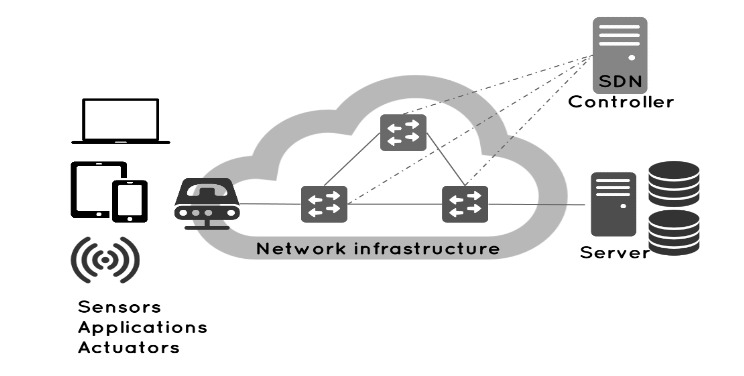
\includegraphics[width=10cm,height=8cm]{media/sdn.jpeg}
\centering
\caption{Software Defined Network}
\end{figure}
In order to connect with the underlying hardware infrastructure and govern traffic on a network, Software-Defined Networking (SDN) requires software-based controllers or application programming interfaces (APIs). The traditional network paradigm, which regulates network traffic using specialised hardware devices like switches and routers, is different from this one. SDN uses software to establish and manage virtual networks as well as traditional hardware.
\\
\subsection{NodeMCU}
\begin{figure} [H]
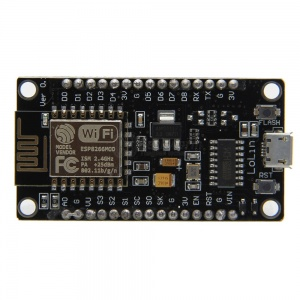
\includegraphics[width=10cm,height=8cm]{media/Esp8266.jpg}
\centering
\caption{ESP8266 Wifi Module}
\end{figure}
The open-source hardware and software platform is called NodeMCU, which stands for Node Microcontroller Unit. This will facilitate the movement of data and objects through WiFi.
A low-cost Wi-Fi microchip with built-in TCP/IP networking software and a microcontroller is called the ESP8266. This little gadget enables easy TCP/IP connections and Wi-Fi network connectivity for microcontrollers. Numerous hackers were drawn to investigate the module, the chip, and the software on it because of its extremely cheap cost and the fact that it had so few external components, which suggested that it would ultimately be very affordable in bulk.

\subsection{OLED}
The SSD1306 single-chip CMOS OLED/PLED driver with controller is a dot-matrix graphic display system for organic or polymer light-emitting diodes. There are 64 commons and 128 segments in it. This IC is designed for Common Cathode OLED displays. Less extra components and power are needed because to the oscillator, display RAM, and contrast control that are included into the SSD1306. There are 256 distinct brightness levels available.
\begin{figure} [H]
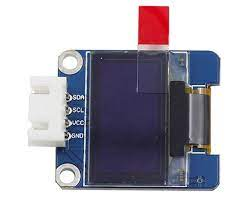
\includegraphics[width=8cm,height=6cm]{media/oled.jpg}
\centering
\caption{OLED Display}
\end{figure}
It is suitable for many compact, portable applications, such as smart watches, real-time photo displays from smart car cameras, battery management tools, etc. The OLED display has good contrast in low light since it doesn't have a backlight. The OLED display uses less electricity than traditional displays because its pixels only use energy when they are turned on. The device we're utilising here uses the I2C protocol to talk to the Arduino and only has four pins. Some versions have an additional RESET pin. Other OLED displays use SPI communication to communicate with one another.
\subsection{DHT11 Sensor}
\begin{figure} [H]
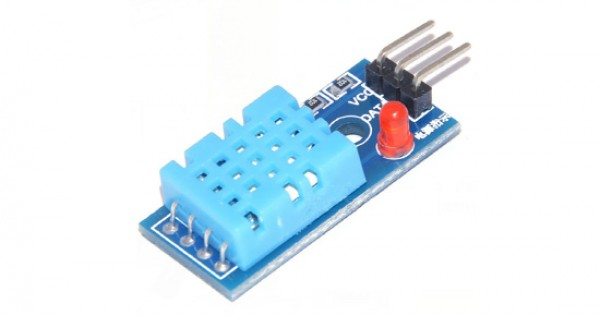
\includegraphics[width=8cm,height=6cm]{media/DHT11module.jpg}
\centering
\caption{DHT11 Sensor}
\end{figure}
It is a digital sensor that measures humidity and temperature. The thermistor and capacitive humidity sensor detect the air and provide data. DHT11 is composed mostly of three parts. The first is a resistive type humidity sensor that provides a reading of the relative humidity. The second is a thermistor with a negative temperature coefficient (NTC), whose purpose is to gauge the target area's temperature. The third component is an 8-bit microcontroller that creates a single digital signal from the received analogue temperature and humidity values. The level of moisture in the air is known as humidity. Even though the temperature is low, individuals may still feel the heat because of the high humidity. Thus, during such periods when certain circumstances exist, humidity values make sense.
\\
\subsection{Application of IOT}
\subsubsection{Smart Agriculture}
Food is essential to life and is necessary for survival. Unfortunately, although people go hungry in less developed nations like America and Chad. Better farming techniques, which can be improved via IoT, are one approach to feed everyone. This can be accomplished only by collecting data for a plantation, like soil health, daylight levels, grain form, flood composition, etc. from different sources, including such plantation detectors, space probes, weather forecast channels, etc., by using this information to learning algorithms and the industrial iot to generate key suggestions for each plantation that will maximise the seeding operation, irrigated agriculture stages required, nutrient quantity, etc.
\subsubsection{Smart Healthcare}
IoT has several uses in the healthcare sector, enabling clinicians to remotely monitor patients through a network of linked gadgets and devices without having to be in close proximity to them. This is quite beneficial if the patients don't have any serious problems or communicable diseases like COVID-19 right now. One of the most well-liked IoT applications is the use of robots in healthcare. These include surgical robots, which can aid surgeons in executing procedures more quickly and precisely. Robots that use high-intensity UV light to swiftly and completely clean surfaces are also available.
\subsubsection{Smart Retail}
Customers may increase their excitement about buying by utilising cutting-edge technology, such as IoT, of course. IoT may be used by retail establishments in a variety of ways to improve both the consumer and employee experience of shopping. IoT may be utilised to manage inventory, enhance business operations, lower theft and shoplifting, and avoid long lines at the cash registers. The Amazon Go shops, which offer an IoT-enabled shopping experience, are a perfect illustration of this. These retailers use IoT to monitor every product they sell, allowing consumers to just pick up what they want and leave the store without waiting in line at the register.\\
\subsection{Real-time Applications}
\begin{enumerate}
    \item \textbf{Health Monitoring for ICU Patients:} With this system it is helpful to monitor the patient's ECG, Body temperature, and even it is helpful to see the room temperature.
    \item \textbf{Rural Community Health Centres:} Specialty providers are sometimes difficult to find, pay for, or keep in rural healthcare institutions. This technology expands the range of services available to patients in rural areas by providing rapid access to a remote specialist without the need for the patient to travel or wait for an appointment.
    \item \textbf{Accurate Results with less staff:} The operating costs of the hospital will be reduced with the aid of our equipment. By delivering a vital reading every minute, our gadget would undertake patient monitoring.
\end{enumerate} 
\subsection{Organisation of the Project Report}
The project report is organized as given below: We talk about the problem statement and our solution in Chapter (2). The same chapter also deals with the other existing technology and the proposed solution. The Chapter that follows i.e. Chapter (3) consists of the details on the literature survey of the papers to the problem statement.  We outline the system architecture in Chapter (4) using a system model and data flow diagram. The requirements and specifics for implementing the suggested system are provided in the next chapter, Chapter (5), together with the technological stack that was employed in the project. In Chapter (6), we discuss the end result of the project. The paper's conclusion is included in Chapter (7), which also mentions future enhancements. The Appendix contains all of the additional supporting data as well as the source code. \newpage
  \pagestyle{fancy}
  \thispagestyle{empty}
  \thispagestyle{plain}
   \fancyhf{}
  \lhead{ESPAsync Web Server to Control Multiple Sensor Reading Using NodeMCU $|$}
  \chead{}
  \rhead{Batch No.: 63}
  \rfoot{Page \thepage \hspace{1pt} of \pageref{LastPage}}
  \lfoot{Dept. of CSE, DSCE}
\renewcommand{\footrulewidth}{0.4pt}% 
\normalsize
\section{Chapter 2: Problem Statement and Proposed Solution}
\subsection{Problem Statement}
To build a web server that is connected to NodeMCU using SDN which retrieves the data from the sensor. \\
\subsection{Existing Systems}
In the existing system there is a need to go to a specific patient's room and have to check the reading of temperature.There is a need for manual work and manpower to check the reading of temperature and humidity and ECG etc.

Here in an existing system there are no multiple sensors available and if we attach also the out of sensors are not uniformed and managed.In this system there are synchronous web servers where the signals are sent continuously Where the man power is needed to check the multiple sensor signals and values.
The sensor values should be checked in the LED only every time where there is no efficiency of memory and time. The sensor operations are very hard to control and getting values from different sensors is also difficult.It is difficult to identify the values of different sensors.In existing systems there is no proper flatform to check. The readings of the Sensors And the sensor readings are not stored properly.
\\
\subsection{Proposed Solution}
In the proposed system there is less manpower required to check the temperature and humidity. And it will show the reading wherever you will be connected to that network. It will be easy to see the temperature, humidity, and ECG of the human body.

The proposed solution uses how to create an asynchronous web server through which we could control multiple outputs from the ESP8266 development board. We are exploring the MQTT protocol in this project. We are using multiple sensors and connected to our NodeMCU. From that user can get this sensor data configuration of modelling like client and server, NodeMCU. In this we will create one web page that will connect to NodeMCU ESP8266 through wifi. For that NodeMCU multiple sensors will be connected.
\\
To create a web server that makes it simple to create an asynchronous web server. There are various advantages to creating an asynchronous web server. 
\textbf{1.} Work with several connections at the same time. \\

\textbf{2.} When you send the response, the server begins processing it in the background, leaving you free to handle new connections straight immediately. \\

\textbf{3.} Handle templates with a simple template processing engine. \\

\subsection{System Requirements} 
\begin{itemize}
    \item \textbf{Processor:} Intel Core i5 8th Generation, 2.4 GHz processor
    \item \textbf{Storage:}  1 TB storage
    \item \textbf{RAM:}  8 GB RAM  
    \item \textbf{OS Version:} Windows 10 
    \item \textbf{The system specifications are as follows:} Arduino IDE, Stable Internet Connection
\end{itemize}
\newpage
  \pagestyle{fancy}
  \thispagestyle{empty}
  \thispagestyle{plain}
  \fancyhf{}
  \lhead{ESPAsync Web Server to Control Multiple Sensor Reading Using NodeMCU $|$}
  \chead{}
  \rhead{Batch No.: 63}
  \rfoot{Page \thepage \hspace{1pt} of \pageref{LastPage}}
  \lfoot{Dept. of CSE, DSCE}
\renewcommand{\footrulewidth}{0.4pt}% 
\normalsize
\section{Chapter 3: Literature Survey} 
\hfill \\
\textbf{\emph {A. Q. Yan, W. Huang, X. Luo, Q. Gong, and F. R. Yu, “A multi-level DDoS mitigation framework for the industrial Internet of Things,” IEEE Commun. Mag., vol. 56, no. 2, pp. 30–36, Feb. 2018.}}

This research looks at analysing the perception layer, network layer, and application layer are the three main layers that make up the IIoT architecture. Due to IIoT's weak defensive system, enormous number of perception nodes, and conventional administration approach, defending against DDoS assaults is challenging. MLDMF is therefore suggested as a defence against DDoS assaults on IIoT. There are three levels in ML DMF as well, matching the three IIoT layers. From bottom to top, these are the levels of edge computing, fog computing, and cloud computing. We think additional IIoT nodes in various locations ought to interact and work together to stop, find, and handle DDoS flooding attacks.\\
Pros: It is designed with great computing power and scalability in mind.\\
Cons: There is not a lot of data, and low-cost services.\\


\textbf{\emph {B. D. Wu, J. Li, S. K. Das, J. Wu, Y. Ji, and Z. Li, “A novel distributed denial-of-service attack detection scheme for software defined networking environments,” in Proc. IEEE Int. Conf. Commun. (ICC), May 2018, pp. 1–6.}}

Network administration is made simpler by Software-Defined Networking (SDN), which divides the control logic plane from the data plane. SDN addresses the issue that traditional networks' static design cannot accommodate the scalable, dynamic computing and storage requirements of modern computing environments, such as data centres. SDN separates the bottom component, which forwards traffic, from the control plane, which decides how to deliver traffic. The high-bandwidth, dynamic nature of today's applications makes SDN an excellent emerging architecture since it is dynamic, controllable, affordable, and adaptive. SDN may be used in a variety of network contexts, including data centres and cloud networks as well as residential and business networks.\\
pros: It provides a lot of scalability and is inexpensive.\\
Cons:  It has a low power consumption and a short battery life.\\ \\


\textbf{\emph {C. C. Li, Z. Qin, E. Novak, and Q. Li, “Securing SDN infrastructure of IoT–fog networks from MitM attacks,” IEEE Internet Things J., vol. 4, no. 5, pp. 1156–1164,Oct. 2017.}}

The Internet of Things (IoT) is playing a more and bigger role in our daily lives, from smart homes to smart cities. By 2020, 12.2 billion M2M connections will exist. Network administrators face a significant problem in managing such a large number of connections. Additionally, IoT objects frequently have resource limitations. They cannot directly support the direct deployment of traditional computing-intensive security measures like encryption and anti-virus software. IoT devices must thus be secured with the aid of the network infrastructure. Traditional networks are no longer appropriate for the IoT in such situations. In contrast, software-defined networking (SDN) offers a number of novel characteristics, including network programmability and centralised control.\\
Pros: It has a low cost and a great scalability.\\
cons: It does not take into account long processing times.\\

 
\textbf{\emph {D. Y. Qiu and M. Ma, “Secure group mobility support for 6LoWPAN networks,” IEEE Internet Things J., vol. 5, no. 2, pp. 1131–1141, Apr. 2018.}}

A potential solution for the Internet of Things (IoT) is IPv6 over Low Power Wireless Personal Area Networks (6LoWPAN), which allows IP connection for devices with limited energy capabilities and permits millions of these IP-based resource-constrained devices to connect to the open Internet. Supporting mobile devices is necessary due to the rising demand for accessibility to different network services whenever and wherever needed. Mobile health monitoring systems, made up of several kinds of 6LoWPAN-based sensors, were created to enable real-time monitoring of distant patients without the use of costly wired cords.\\ \\
Pros: It delivers low cost and secure communication in IoT devices.\\
\\ 
cons: It has less immunity to interference than wifi or Bluetooth devices.
 \\ \\ \\ \\
 
\textbf{\emph {E. D. B. Rawat and S. R. Reddy, “Software defined networking architecture, security and energy efficiency: A survey,” IEEE Commun. Surveys Tuts., vol. 19, no. 1, pp. 325–346, 1st Quart., 2017.}}

The infrastructures for information and communication technology (ICT) are constantly growing as a result of the rise in the number of Internet-of-Things (IoT) and cyber-physical system devices and applications. SDN is a technology that is thought to be capable of effectively controlling the complete network and converting a complicated network design into one that is simple and controllable. Recent research has demonstrated that conventional networks, which are vertically linked and have a complicated, difficult-to-manage structure, are unable to meet the demands that are increasing. Traditional networks lack flexibility for changing network environments and can only implement vendor-specific regulations.
 \\
Pros: It provides scalability, fault tolerance, energy efficient, resource utilisation, cost effective, highly accurate, dynamic management.
 \\
Cons: It has a complex architecture, delay, limited flow entries, more memory consumption, high processing time.
\\ \\
 
\textbf{\emph {F.Fatih Bakir, Rich Wolski, Chandra Krintz Univ. of California, Santa Barbara Gowri Sankar Ramachandran Univ. of Southern California, “Devices-as-Services: Rethinking Scalable Service Architectures for the Internet of Things” (2019).}}

These things are best represented as servers, from which cloud-based software packages are built. We look at how this "flipped" IoT client-server architecture may affect server discovery, resource consumption, and authentication. We find that this architecture can provide quick response and energy efficiency by integrating capability-based security with an edge-aware registry.
 \\ \\
pros: It has feasible, very little overhead and power consumption.
 \\ \\
cons: It has failure to consume power, low cost.
\\ \\ \\ 
 
\textbf{\emph {G.  W. Zhou, Y. Jia, A.   Peng, Y. Zhang, and P. Liu, “The effect of IoT new features on security and privacy: New threats, existing solutions, and challenges yet to be solved,” IEEE Internet Things J., vol. 6, no. 2, pp. 1606–1616, Apr. 2019.}}

The Internet of Things (IoT) is a rapidly gaining in popularity technology that allows actual objects, such as cars, appliances, and other household items, to interact and even speak with one another. It has been extensively employed in social applications, such as smart homes, healthcare, and industrial automation, as well as in industrial production. While delivering previously unheard-of ease of use, accessibility, and effectiveness, IoT has recently raised serious security and privacy concerns. Although more research is being done to lessen these hazards, many issues are still unresolved.\\
Pros: Malware is being used to exploit numerous IoT devices and high scalability.
 
Cons: It has a complex design, delays, limited flow entries, higher memory consumption, and a long processing time, which has been exploited by attackers.
\\ \\
\textbf{\emph {H. U. Banerjee, C. Juvekar, S. H. Fuller, and A. P. Chandrakasan, “eeDTLS: Energy-efficient datagram transport layer security for the Internet of Things,” in Proc. IEEE Global Commun. Conf. (GLOBECOM), Dec. 2017, pp. 1–6.}}

One of the best protocols for safeguarding the IoT is said to be Datagram Transport Layer Security (DTLS). On resource-constrained IoT sensor nodes, DTLS implementation is particularly costly due to computation and communication overheads. RF communications experimental models and cryptographic computations are used. eeDTLS, a low-energy variant of DTLS that provides the same degree of security as DTLS but consumes less energy, is introduced on the basis of this work. The number of sensor nodes in an Internetwork can vary between tens to thousands.  Because they must operate unsupervised for extended durations but are either rechargeable batteries or rely on harvested energy, these devices are severely energy-constrained.\\
 \\
pros: DTLS offers excellent security guarantees, as well as a high level of scalability and the ability to employ frequency radio communications.
 
cons: Due to computation and communication overhead, DTLS on resource constrained IoT sensor nodes are relatively expensive. The cost of obtaining a sensor node utilizing DTLS is significant, but it provides a low-energy power source.
\\ 
\textbf{\emph {I. N. Maheshwari and H. Dagale, “Secure communication and firewall architecture for IoT applications,” in Proc. 10th Int. Conf. Commun.Syst. Netw. (COMSNETS), Jan. 2018, pp. 328– 335.}}

This technique comprises minimally invasive sensing, transmission, and processing of real-time data obtained from billions of linked devices. They are susceptible to numerous assaults due to their accessibility to the Internet and the limitations of IoT devices, which often have little memory and weak computing power. Because IoT is mostly non-realtime and non-safety critical, the typical security approach for Internet applications is inapplicable. Through IoT devices, communication routes between devices and the back-end system, IoT-specific back-end apps, and back-end data storage, it gives hostile users a new attack surface.
\\ \\
pros: It allows remote smart devices to connect to the internet from anywhere in the world. Sensing, connectivity, and real-time data handling are all part of this technology.\\
 
cons: Security and privacy are two drawbacks. This may be the most serious downside of IoT, as people's privacy is jeopardised as a result of their adoption and use of smart gadgets in their daily lives. 

\newpage
  \pagestyle{fancy}
  \thispagestyle{empty}
  \thispagestyle{plain}
  \fancyhf{}
  \lhead{ESPAsync Web Server to Control Multiple Sensor Reading Using NodeMCU $|$}
  \chead{}
  \rhead{Batch No.: 63}
  \rfoot{Page \thepage \hspace{1pt} of \pageref{LastPage}}
  \lfoot{Dept. of CSE, DSCE}
\renewcommand{\footrulewidth}{0.4pt}% 
\normalsize
\section{Chapter 4: Architecture and Design} 
\subsection{System Architecture}
\subsubsection{System Block Diagram}
This esp8266 will create wireless network with the servers. For that other network other devices can also connect using SSID and password. This SSID and password is for the authentication. The NodeMCU has been set as station. Then client can send the HTTP GET request from the website that has been built. And it will connect to the server that is NodeMCU and it will fetch the data from the sensor and server will show the data in OLED and also it will show the result in webpage. In webpage we have to give IP address for the specific sensor it will fetch the data from the sensor and it will show the output.
\\

\begin{figure} [H]
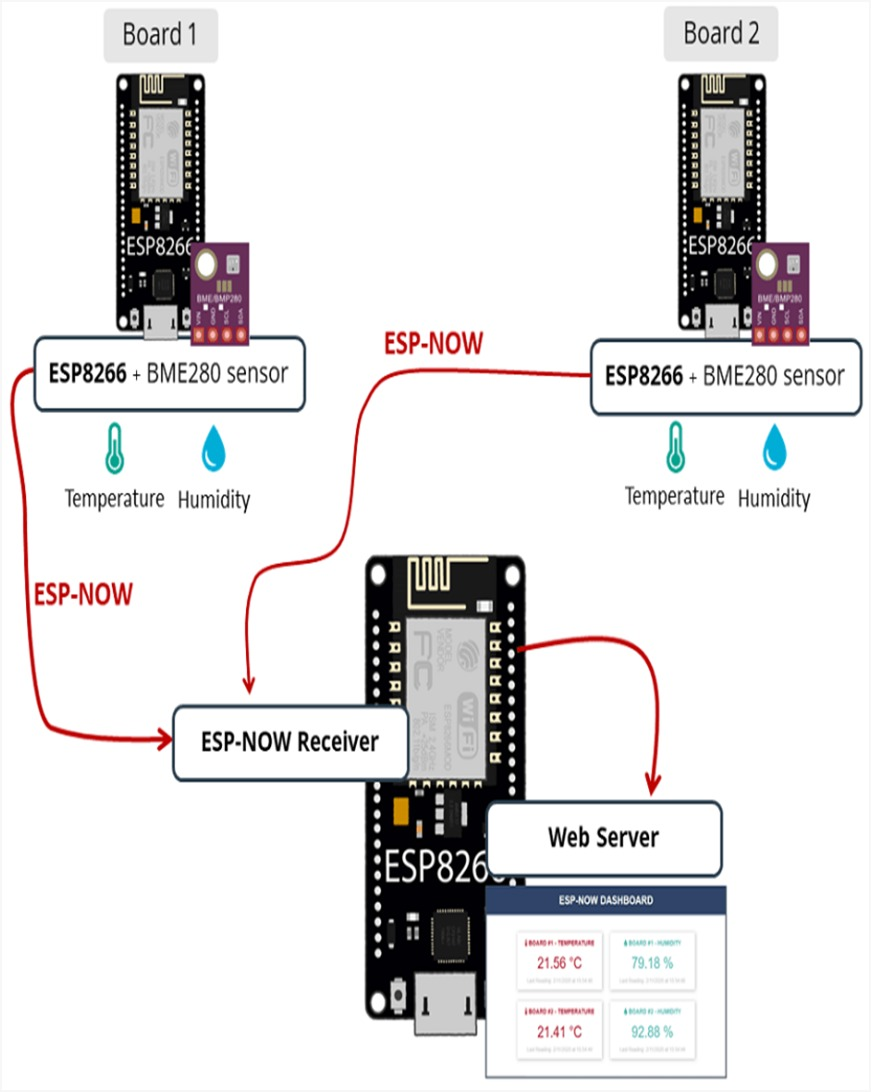
\includegraphics[width=12cm,height=8cm]{media/block.jpeg}
\centering
\caption{System Model}
\end{figure}
\newpage
  \pagestyle{fancy}
  \fancyhf{}
  \lhead{ESPAsync Web Server to Control Multiple Sensor Reading Using NodeMCU $|$}
  \chead{}
  \rhead{Batch No.: 63}
  \rfoot{Page \thepage \hspace{1pt} of \pageref{LastPage}}
  \lfoot{Dept. of CSE, DSCE}
\renewcommand{\footrulewidth}{0.4pt}% 
\normalsize
\subsubsection{Data Flow Diagram}
\begin{figure} [H]
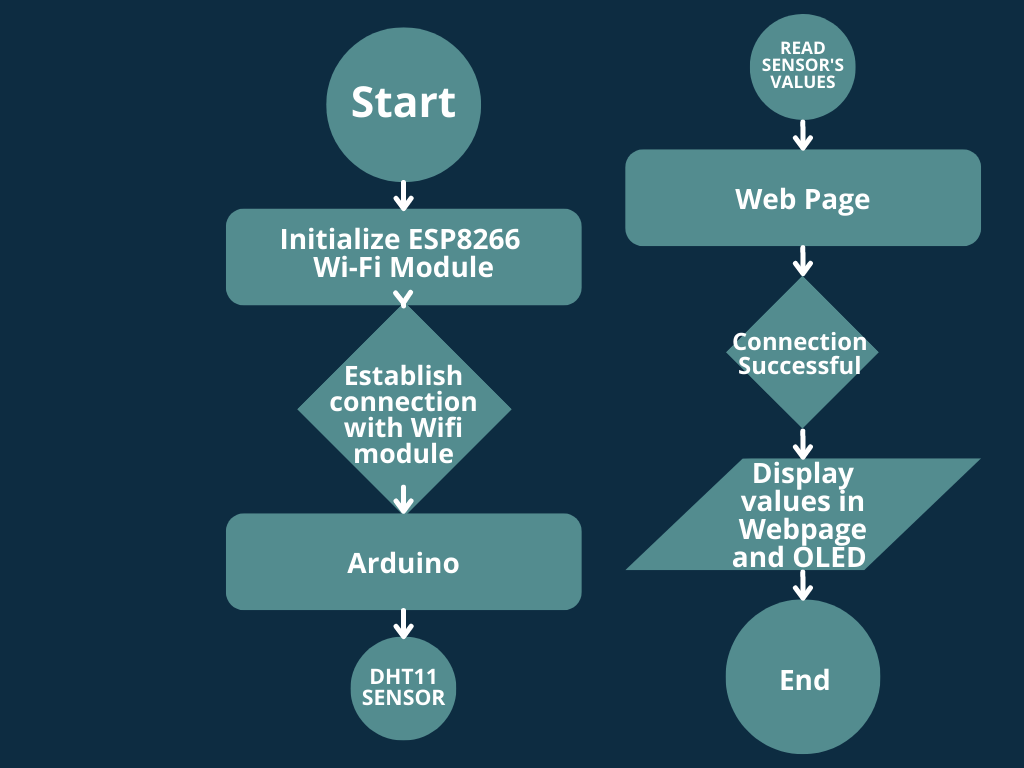
\includegraphics[width=18cm,height=10cm]{media/Data Flow.png}
\centering
\caption{Data Flow Diagram}
\end{figure}
Figure 4.2 represents the Data flow diagram, The wifi module ESP8266 has been configured as TCP/IP client.Once the client sends the request by giving the Authentication through the webpage that webpage will be connected to the NodeMCU and it will go to sensor.The NodeMCU will fetch the data from the sensor and it will show the result in the OLED and webpage. The wifi module will fetch the data based on the IP address that has been assigned to the specific sensor. This information can be representing the Information flow.
\newpage
  \pagestyle{fancy}
  \fancyhf{}
  \lhead{ESPAsync Web Server to Control Multiple Sensor Reading Using NodeMCU $|$}
  \chead{}
  \rhead{Batch No.: 63}
  \rfoot{Page \thepage \hspace{1pt} of \pageref{LastPage}}
  \lfoot{Dept. of CSE, DSCE}
\renewcommand{\footrulewidth}{0.4pt}% 
\normalsize
\newpage
  \pagestyle{fancy}
  \thispagestyle{empty}
  \thispagestyle{plain}
  \fancyhf{}
  \lhead{ESPAsync Web Server to Control Multiple Sensor Reading Using NodeMCU $|$}
  \chead{}
  \rhead{Batch No.: 63}
  \rfoot{Page \thepage \hspace{1pt} of \pageref{LastPage}}
  \lfoot{Dept. of CSE, DSCE}
\renewcommand{\footrulewidth}{0.4pt}% 
\normalsize
\section{Chapter 5: Implementation} 
\subsection{Implementation Platforms}
\subsubsection{Hardware}
\begin{itemize}
    \item \textbf{Processor:} Intel Core i5 8th Generation, 1.80GHz Processor
    \item \textbf{RAM:} 8GB
    \item \textbf{Storage:} 1TB
\end{itemize}
\subsubsection{Software}
\begin{itemize}
    \item \textbf{Operating System:} Windows 10 (64 bit)
    \item \textbf{Software Used:} Arduino, Visual Studio Code, Notepad++
    \item \textbf{Programming Languages:} HTML, CSS, C
\end{itemize}
\subsection{Implementation Details}
\subsubsection{Software for Initialization and Configuration of Hardware }
\begin{figure} [H]
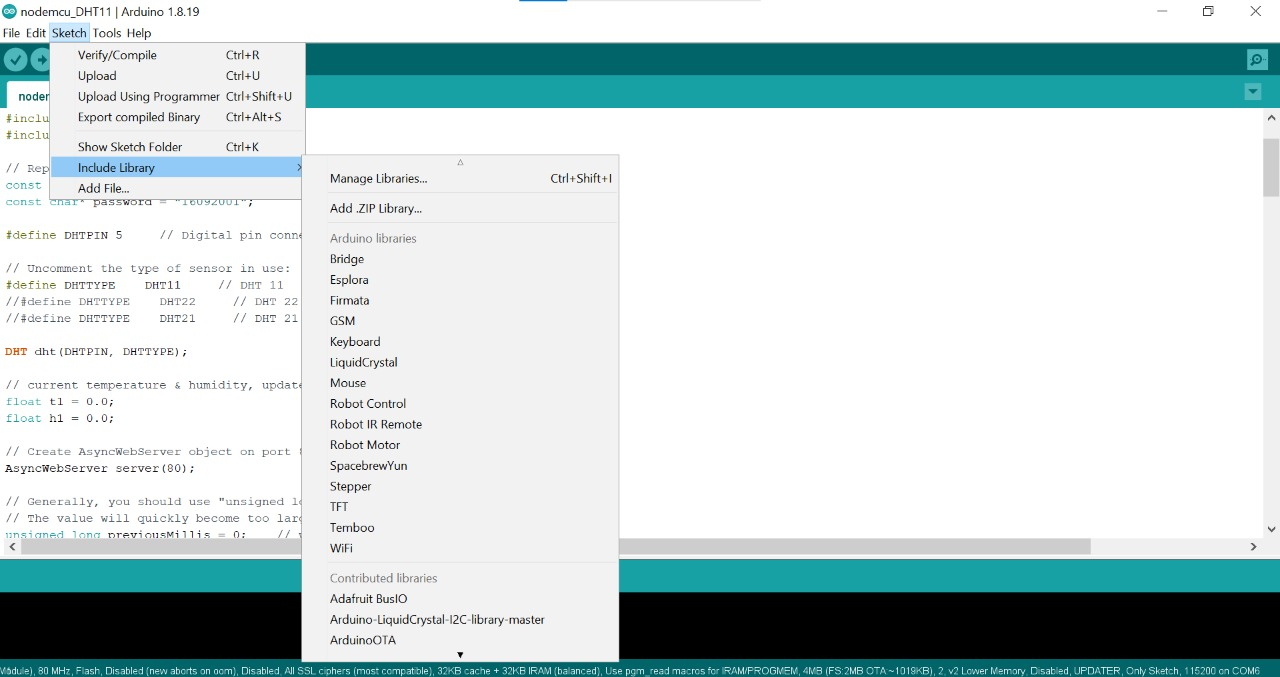
\includegraphics[width=17cm]{media/lib (2).jpeg}
\centering
\caption{Installing libraries using the Arduino IDE}
\end{figure} 
Figure 5.1 depicts how Arduino IDE is used to write program for NodeMCU ESP8266 for fetching the data from the sensor and send that result to the webpage and OLED. First we have checked for the single sensor and integrated with the multiple sensors.
\begin{figure} [H]
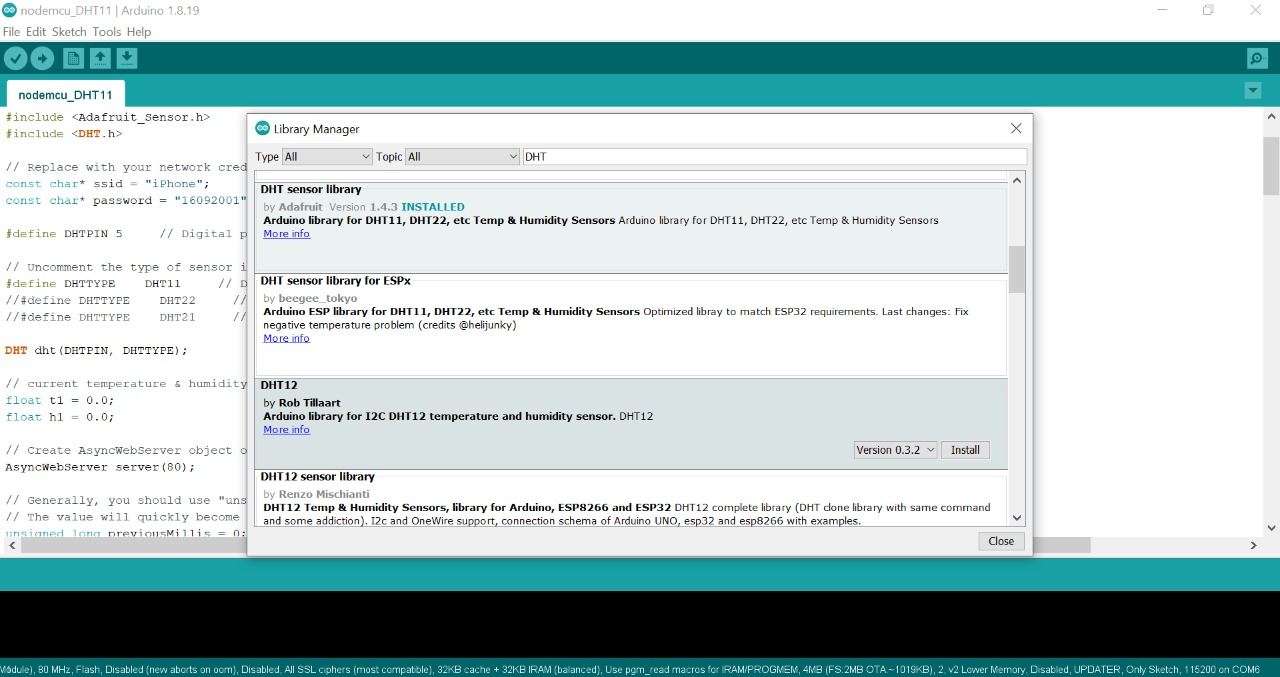
\includegraphics[width=17cm]{media/lib (1).jpeg}
\centering
\caption{DHT Library installation }
\end{figure}
Figure 5.2 Shows include the libraries from Sketch. Click on Include Library and Manage Libraries in the Arduino IDE. The WiFi management libraries can then be installed. Installing the DHT sensor library is as simple as choosing "DHT sensor library by Adafruit Version" and choosing the version you want to use. It is advised to choose the most recent DHT-11 and WiFi management Library versions.
\begin{figure} [H]
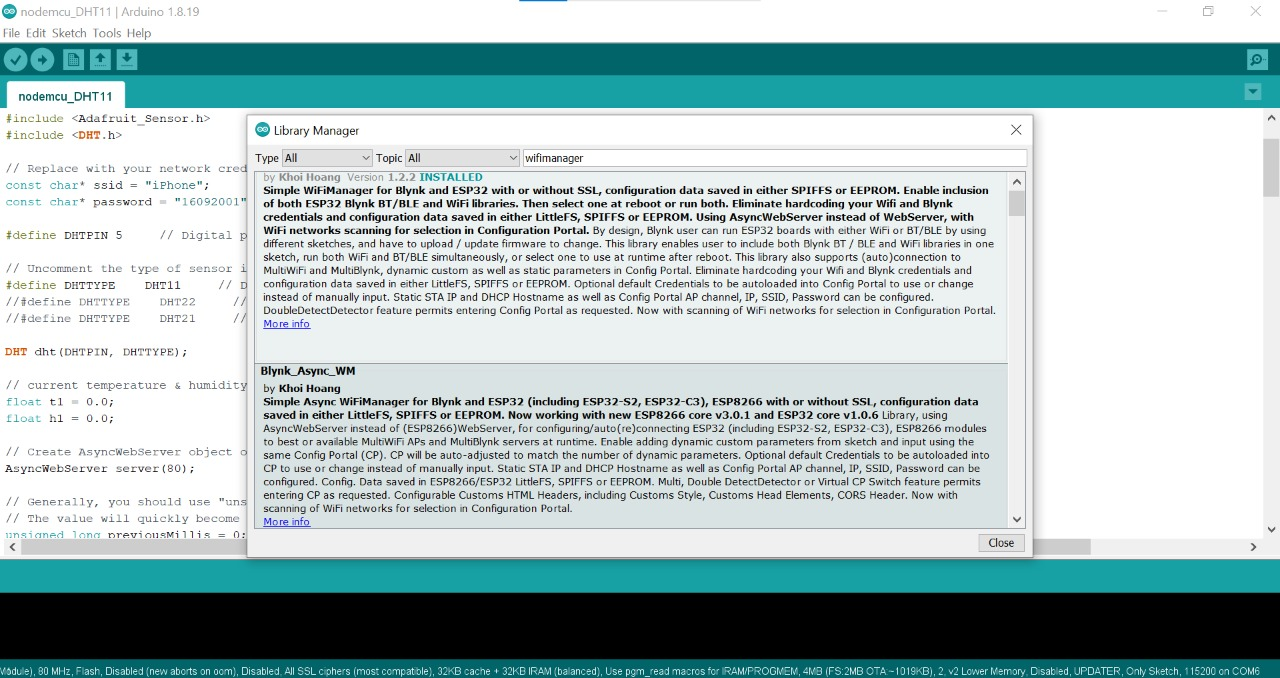
\includegraphics[width=17cm]{media/lib (3).jpeg}
\centering
\caption{WiFi Manager Library installation }
\end{figure}
\subsubsection{Front-end Integration}
In front end integration we have used HTML and CSS for creating web pages.
These requires two Phases. Namely:

1.Login page

2.Sensor output phase :In the Login phase we have And in the login phase we are given SSID and Password. It should match with the original for authentication and there will IP address and Gateway and we have made use of CSS for making Box and aligning.

\newpage
  \pagestyle{fancy}
  \thispagestyle{empty}
  \thispagestyle{plain}
  \fancyhf{}
  \lhead{ESPAsync Web Server to Control Multiple Sensor Reading Using NodeMCU $|$}
  \chead{}
  \rhead{Batch No.: 63}
  \rfoot{Page \thepage \hspace{1pt} of \pageref{LastPage}}
  \lfoot{Dept. of CSE, DSCE}
\renewcommand{\footrulewidth}{0.4pt}% 
\normalsize
\section{Chapter 6: Results}
\begin{figure} [H]
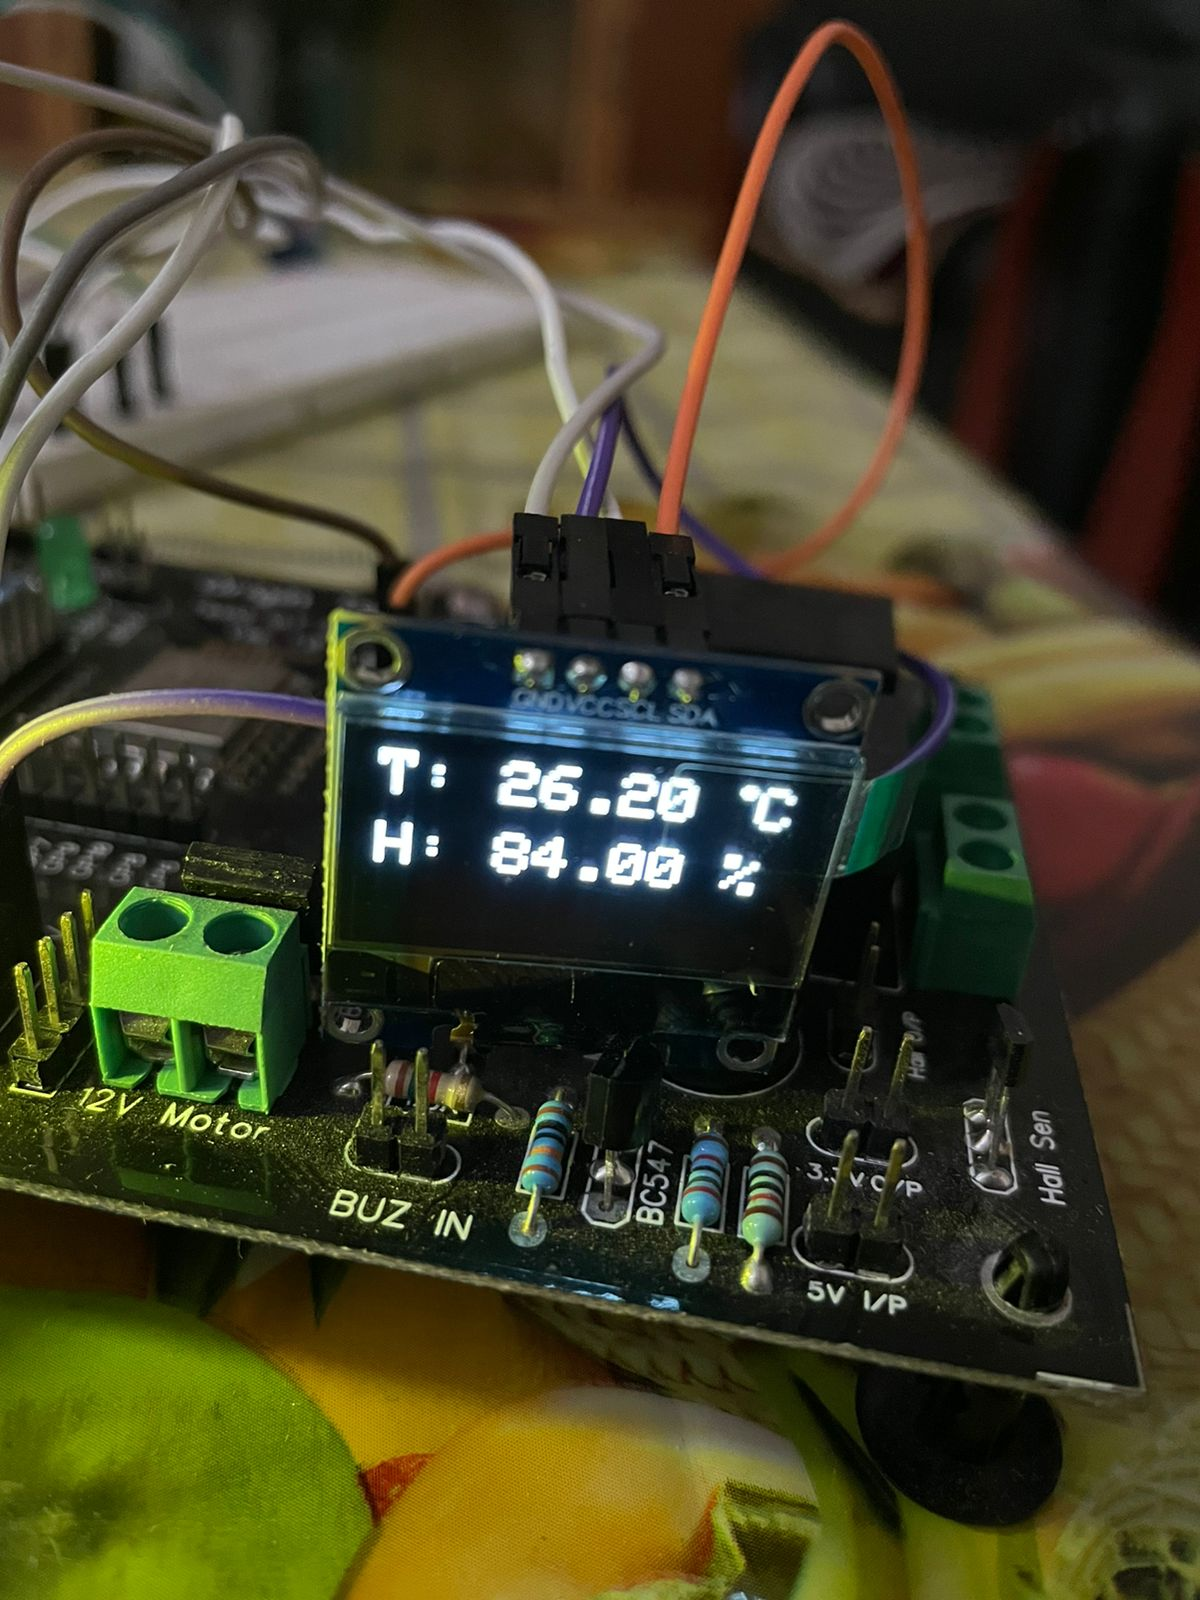
\includegraphics[width=15cm]{media/OLED display.jpeg}
\centering
\caption{OLED Display}
\end{figure}
\begin{figure} [H]
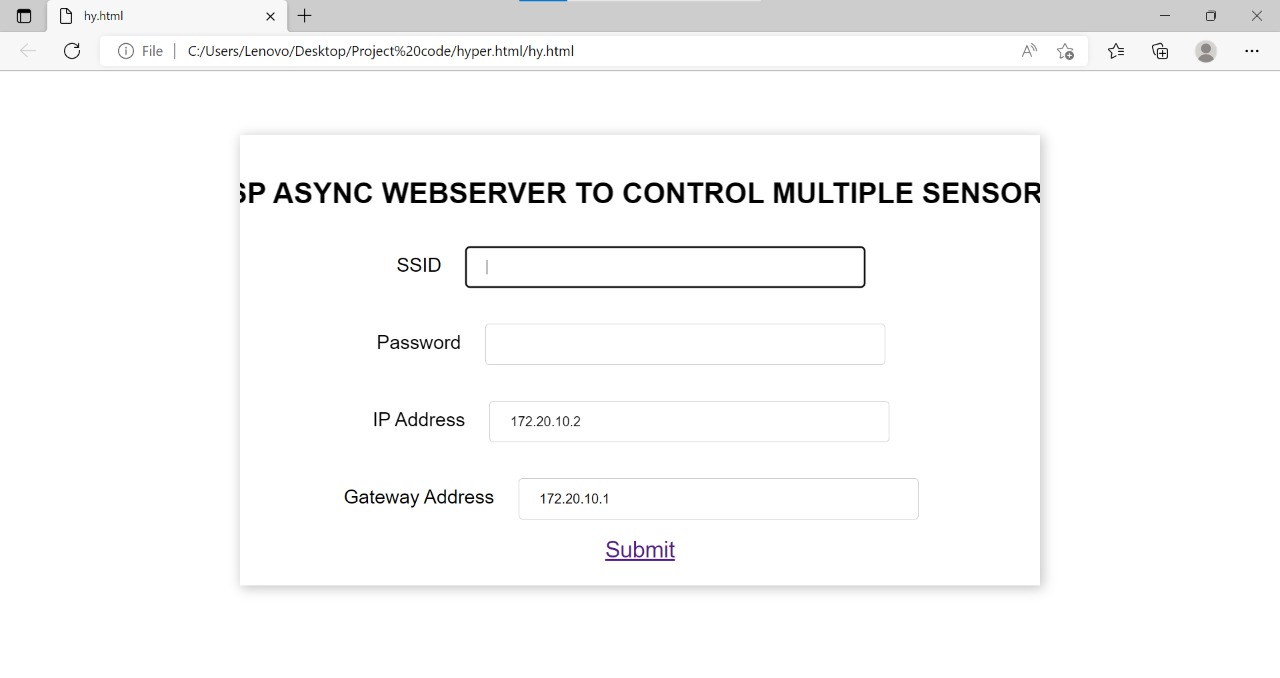
\includegraphics[width=15cm]{media/WebPage.jpeg}
\centering
\caption{Web Page}
\end{figure}
\begin{figure} [H]
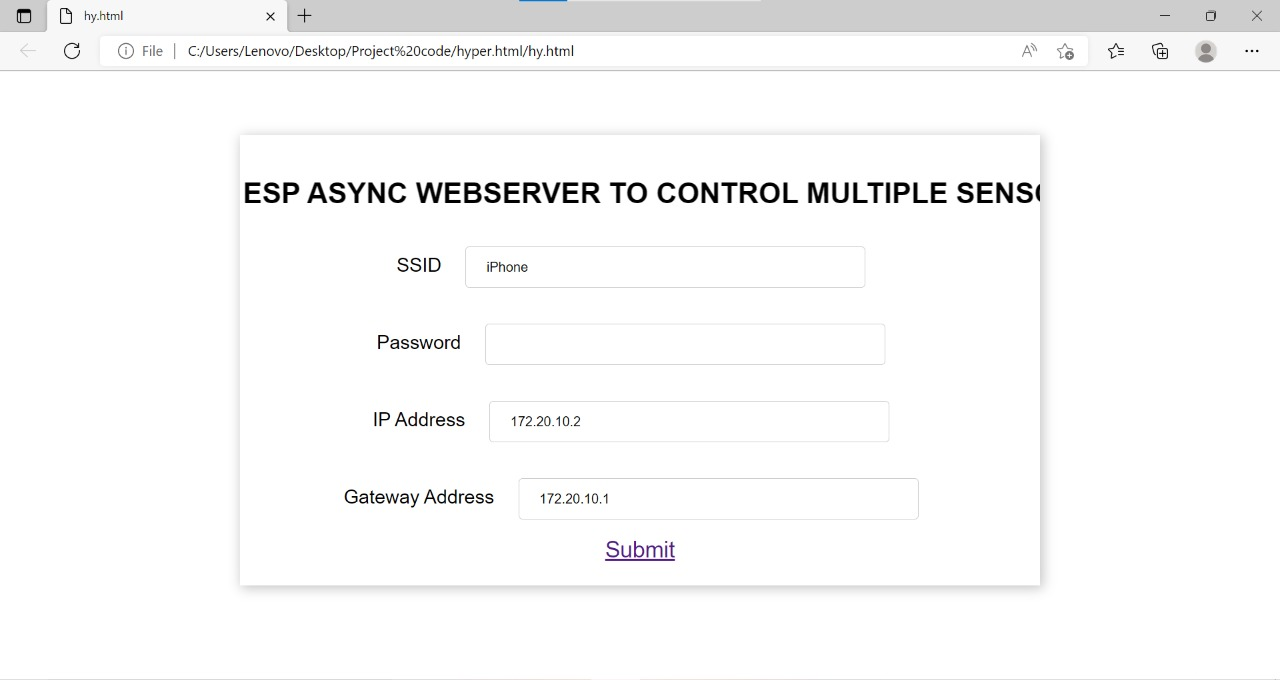
\includegraphics[width=15cm]{media/LoginID.jpeg}
\centering
\caption{Login ID}
\end{figure}
\begin{figure} [H]
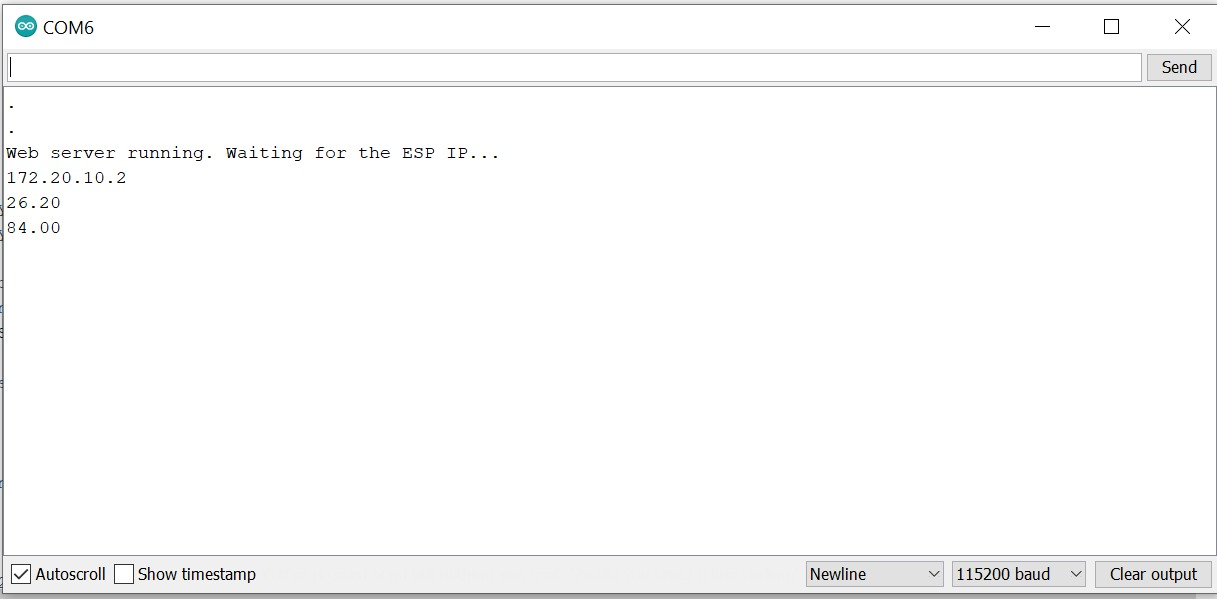
\includegraphics[width=15cm]{media/Sensor1.jpeg}
\centering
\caption{ Arduino Console }
\end{figure}
\begin{figure} [H]
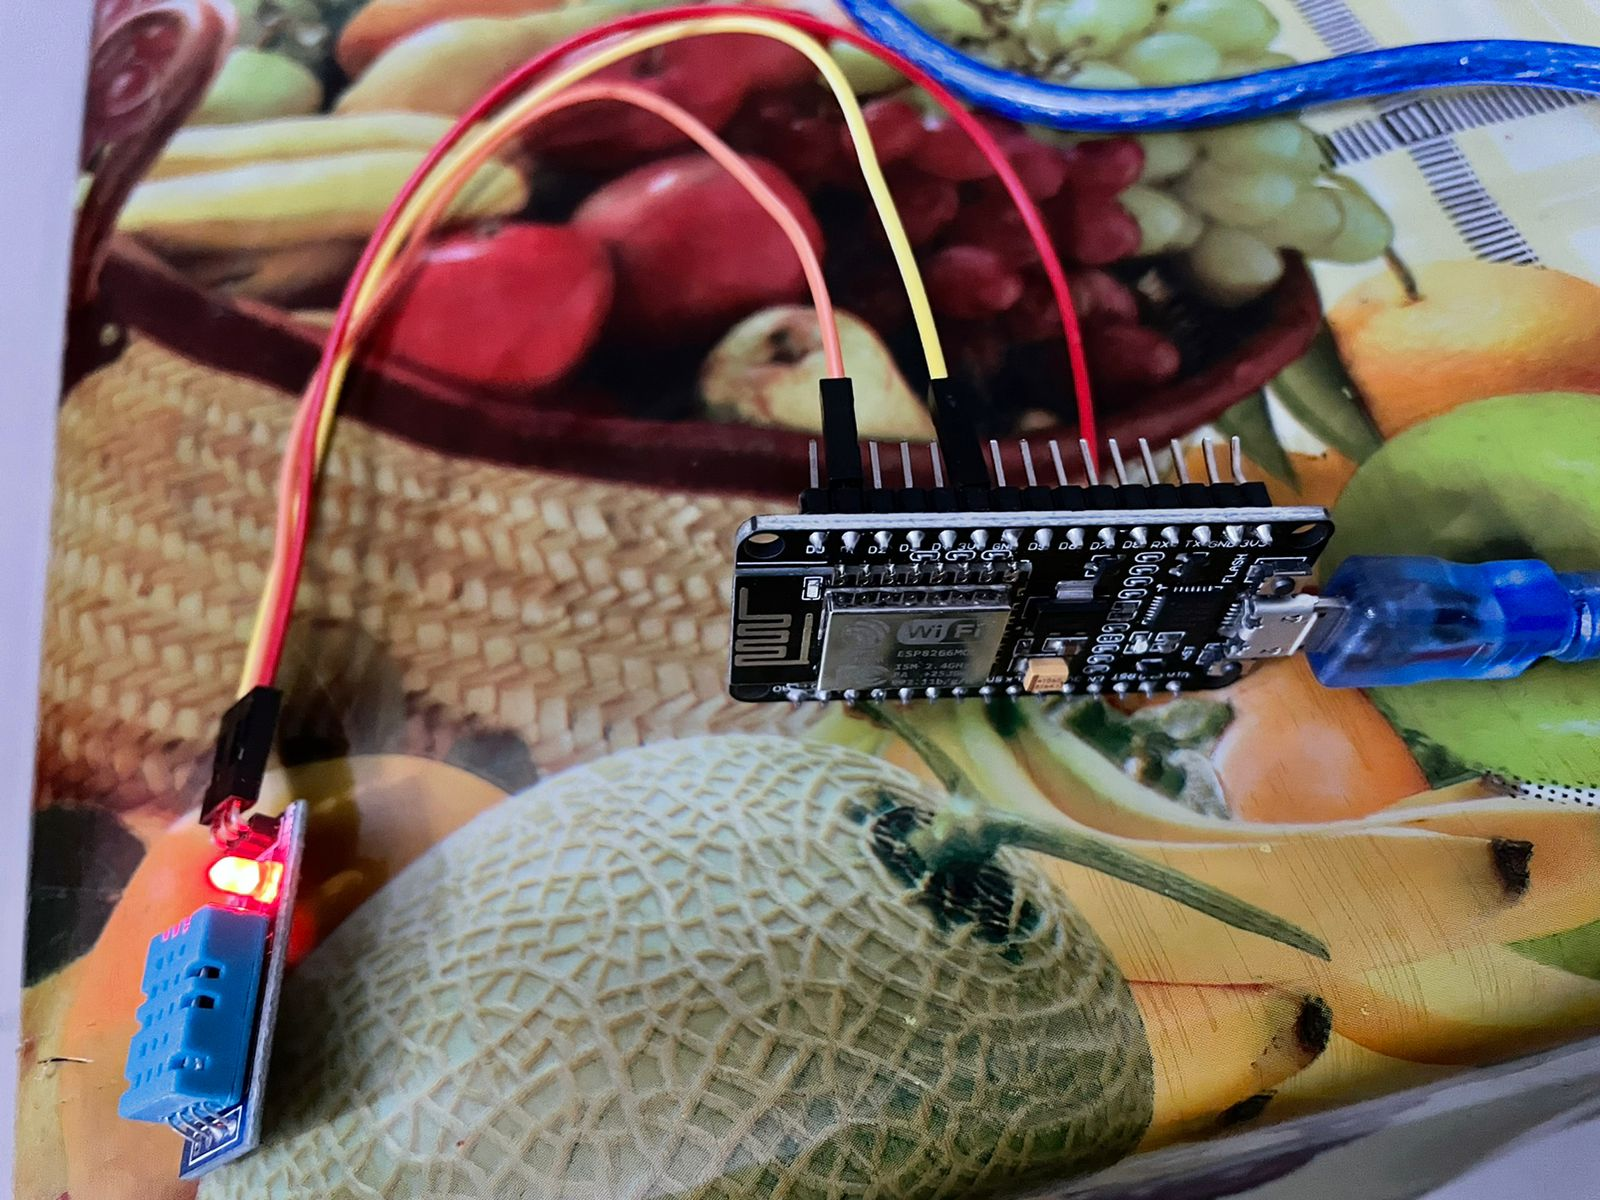
\includegraphics[width=15cm]{media/SensorWeb1.jpeg}
\centering
\caption{Sensor}
\end{figure}
\begin{figure} [H]
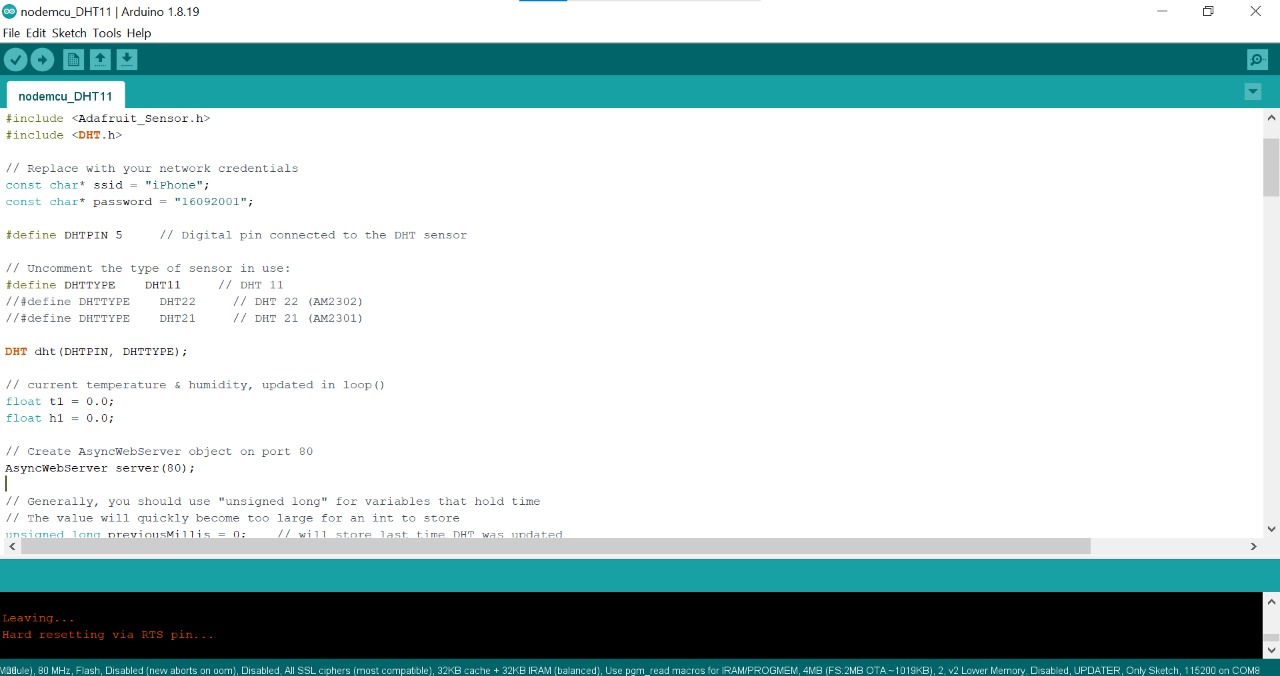
\includegraphics[width=15cm]{media/out (1).jpeg}
\centering
\caption{Compile}
\end{figure}
\begin{figure} [H]
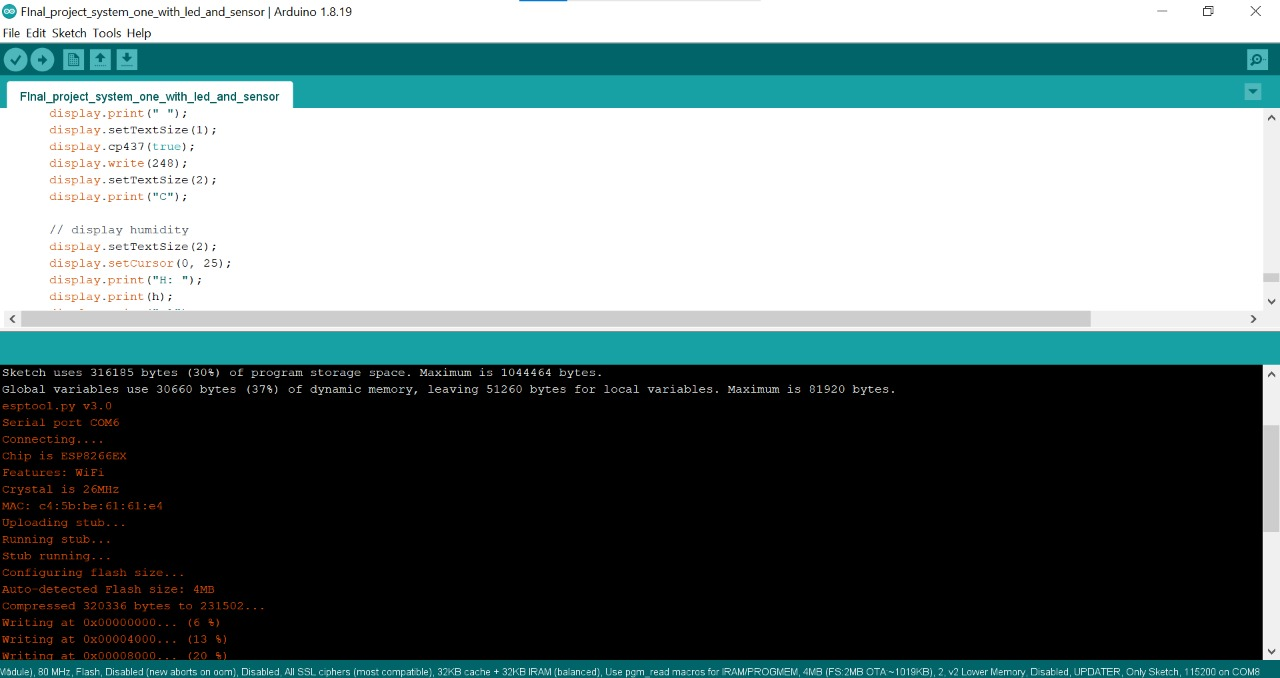
\includegraphics[width=15cm]{media/out (2).jpeg}
\centering
\end{figure}
\begin{figure} [H]
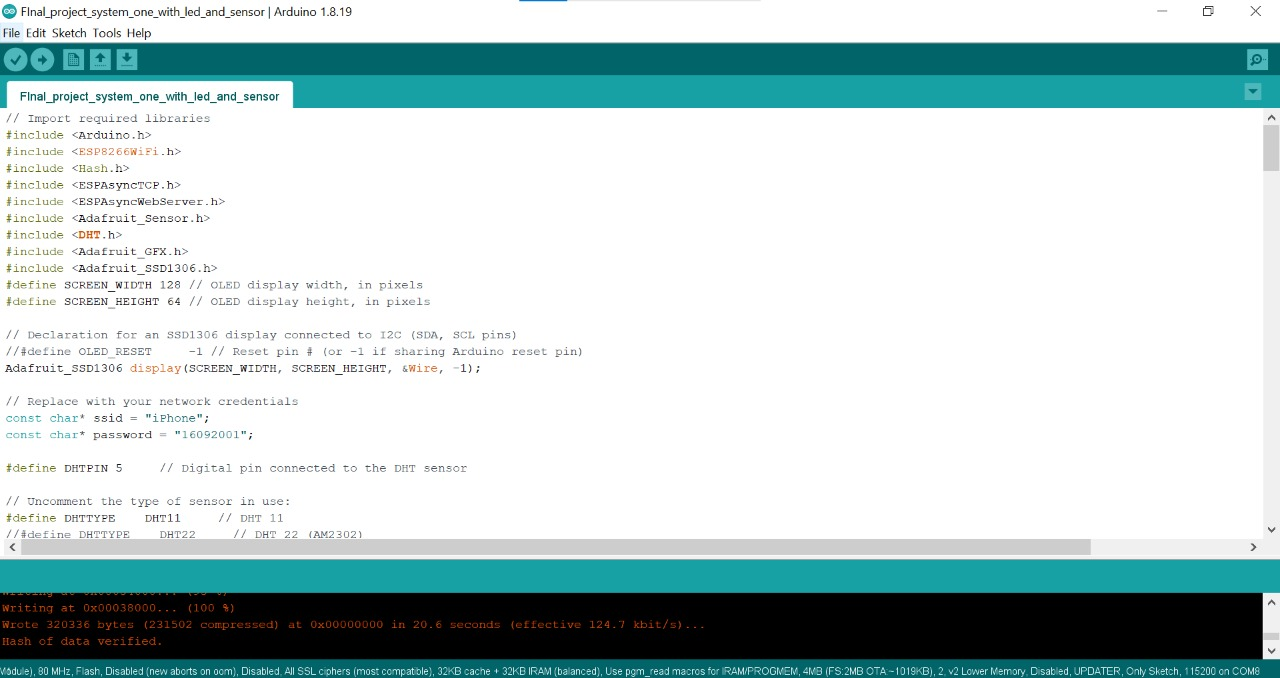
\includegraphics[width=15cm]{media/out (3).jpeg}
\centering
\end{figure}
\begin{figure} [H]
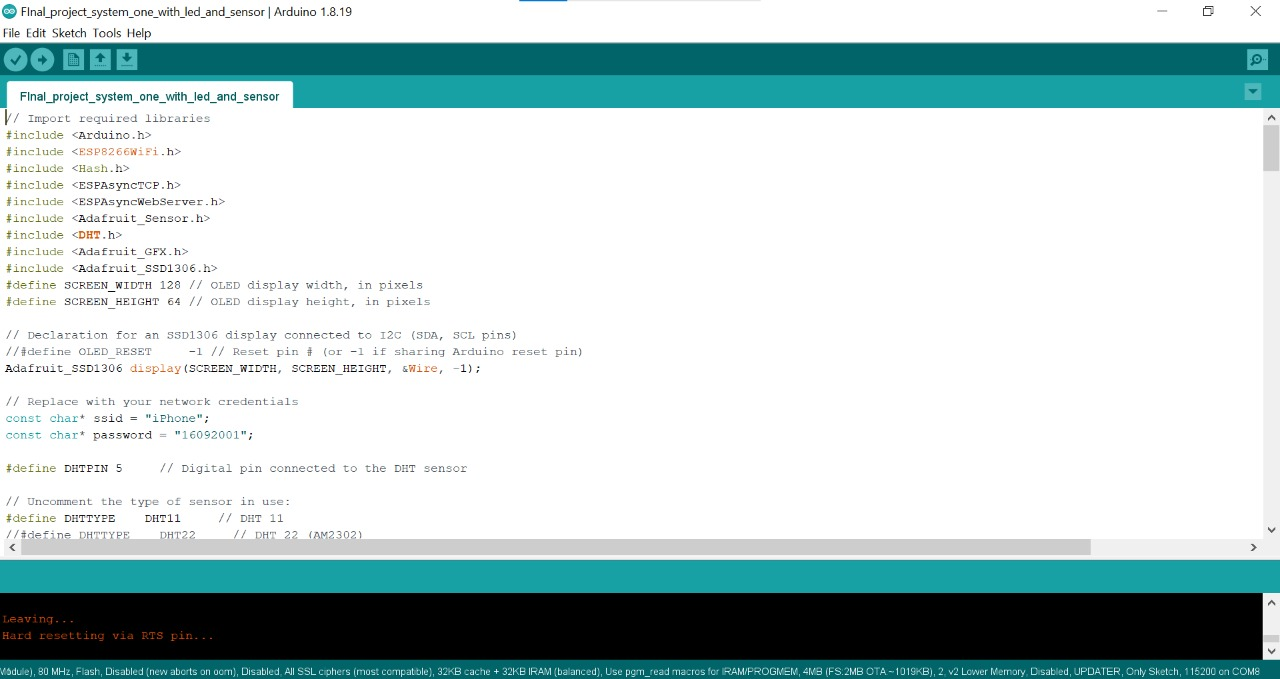
\includegraphics[width=15cm]{media/out (4).jpeg}
\centering
\end{figure}
\begin{figure} [H]
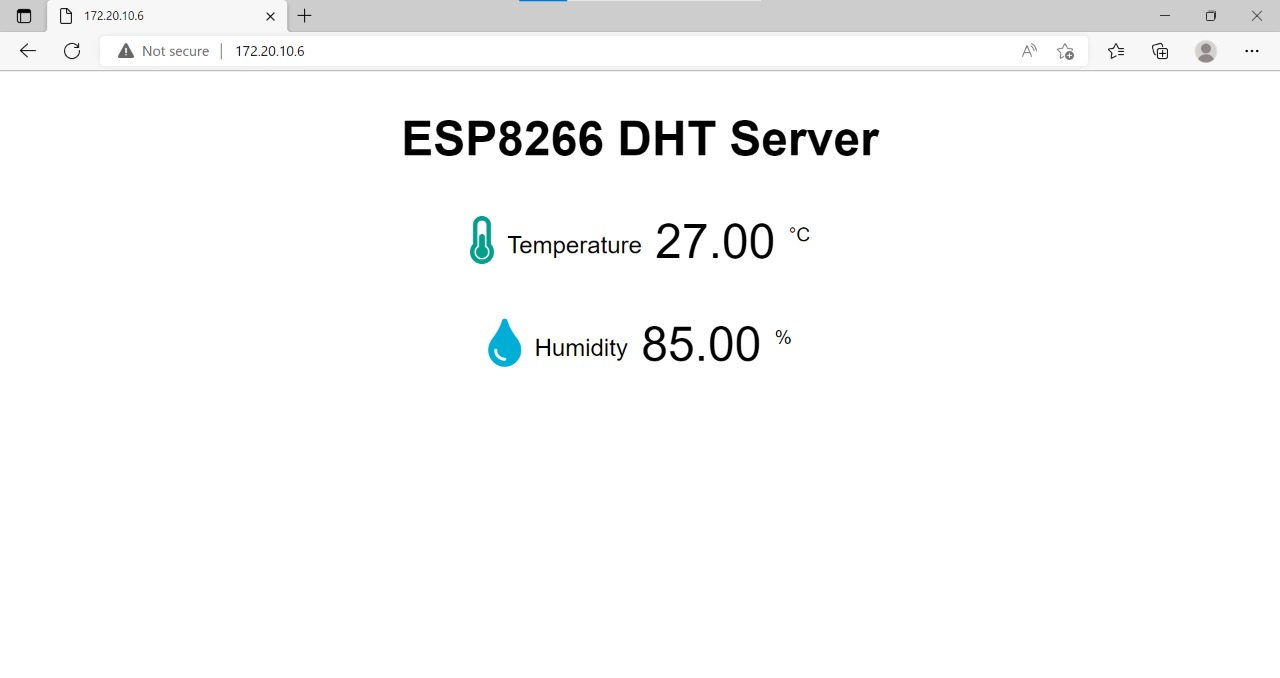
\includegraphics[width=15cm]{media/WebPage Display.jpeg}
\centering
\caption{Sensor Values}
\end{figure}
\begin{figure} [H]
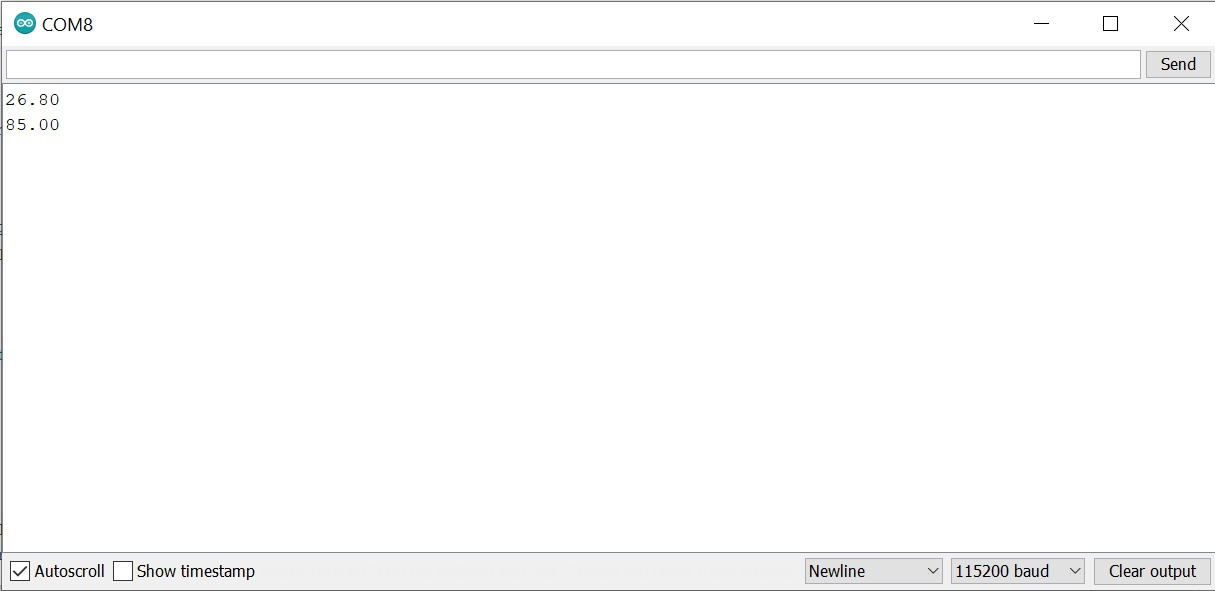
\includegraphics[width=15cm]{media/Sensor2.jpeg}
\centering
\caption{Another Sensor Arduino console}
\end{figure}
\begin{figure} [H]
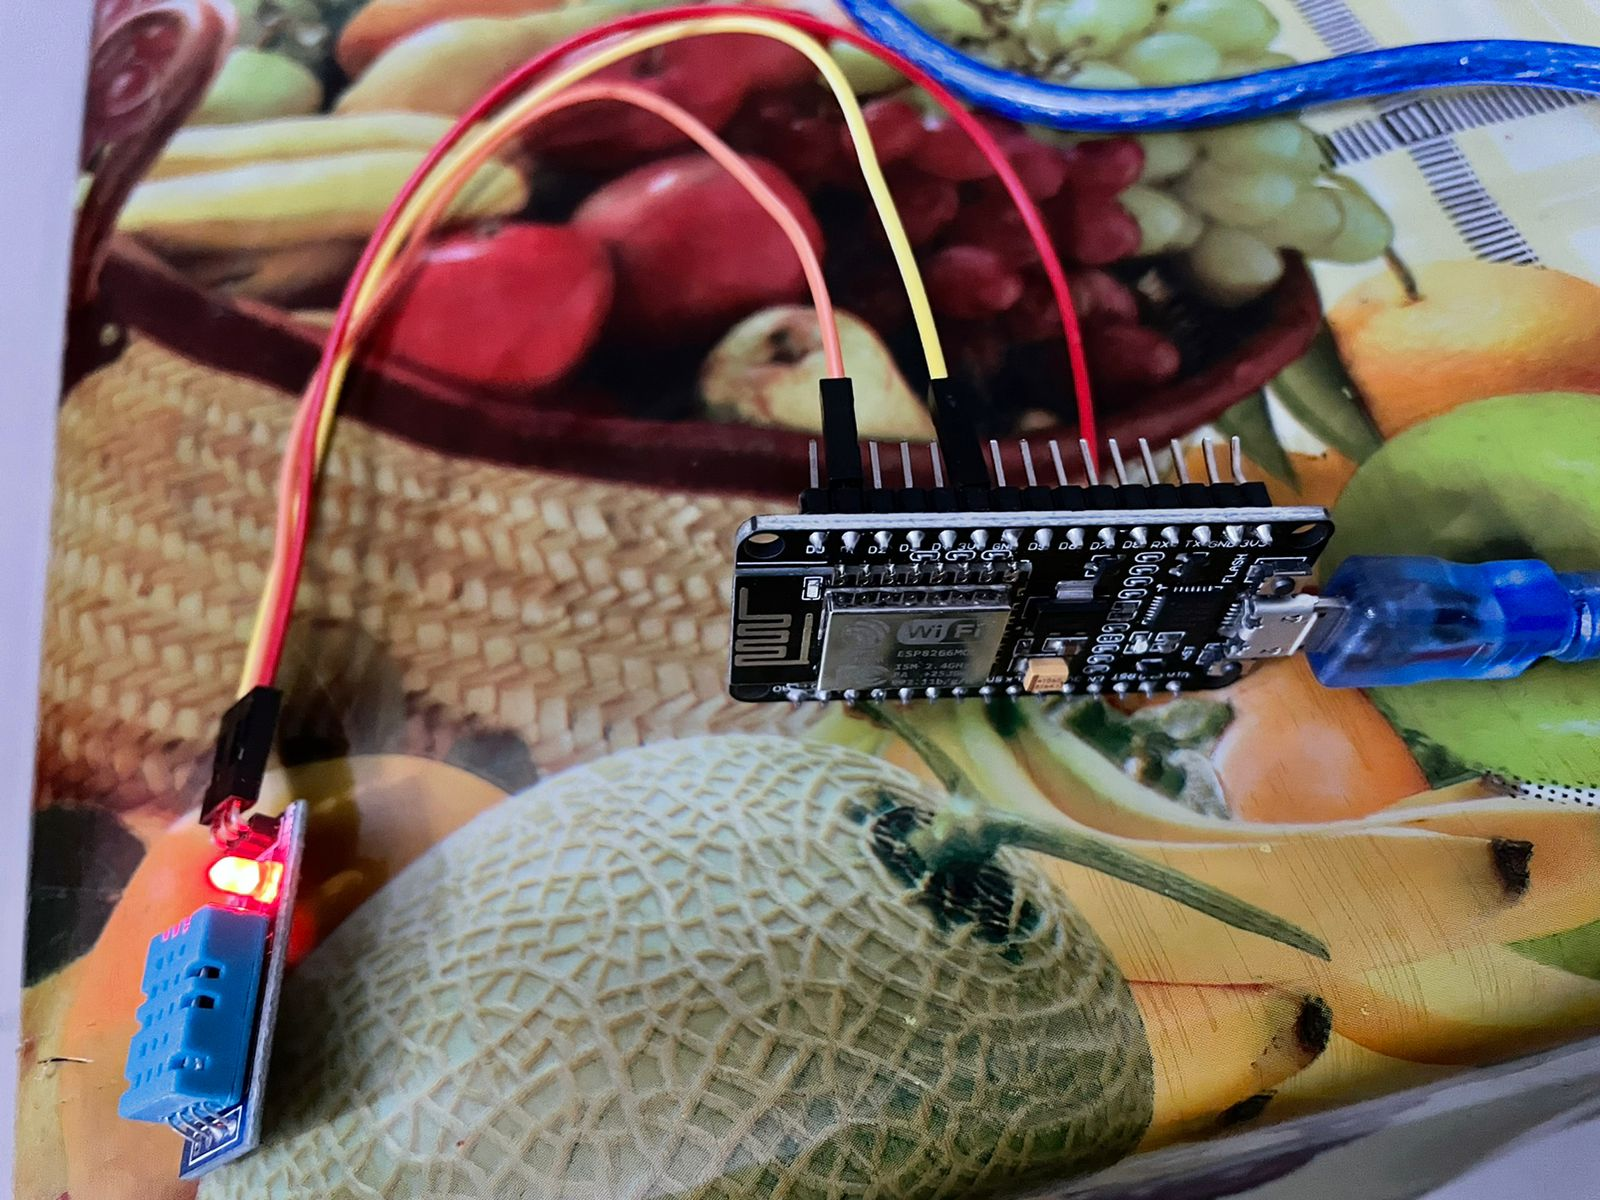
\includegraphics[width=15cm]{media/SensorWeb1.jpeg}
\centering
\caption{Sensor With NodeMCU}
\end{figure}
\begin{figure} [H]
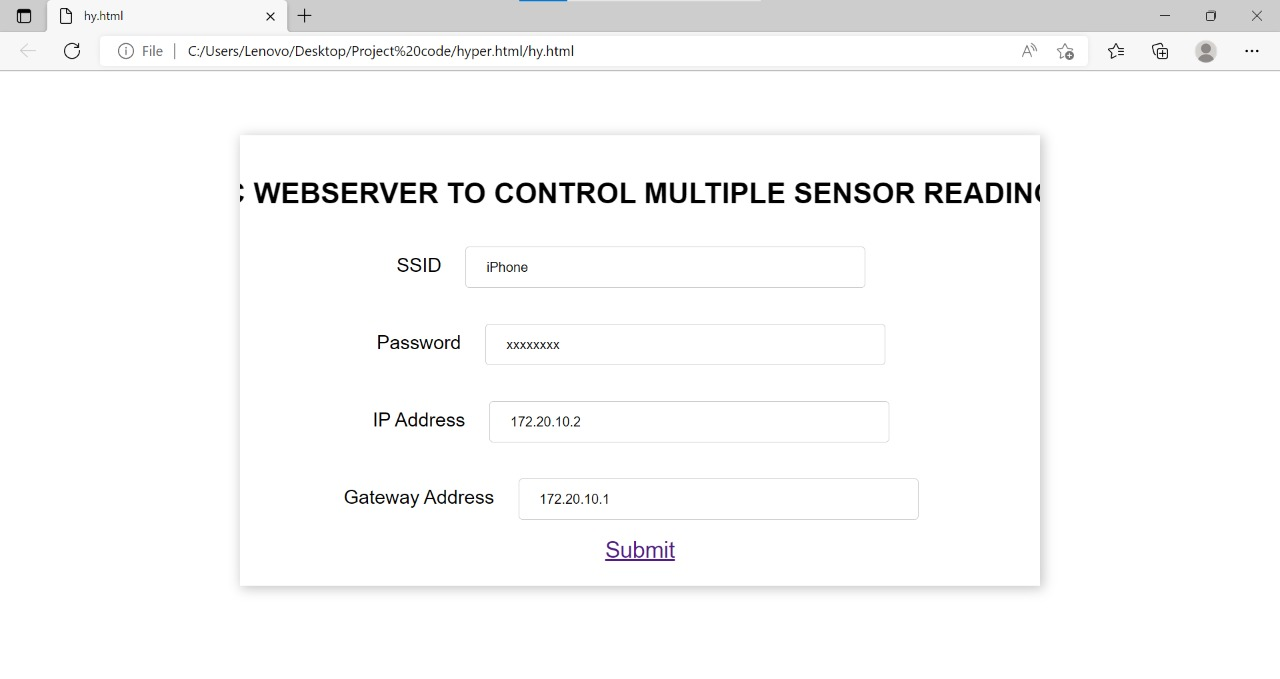
\includegraphics[width=15cm]{media/Login.jpeg}
\centering
\caption{Login Page}
\end{figure}
\begin{figure} [H]
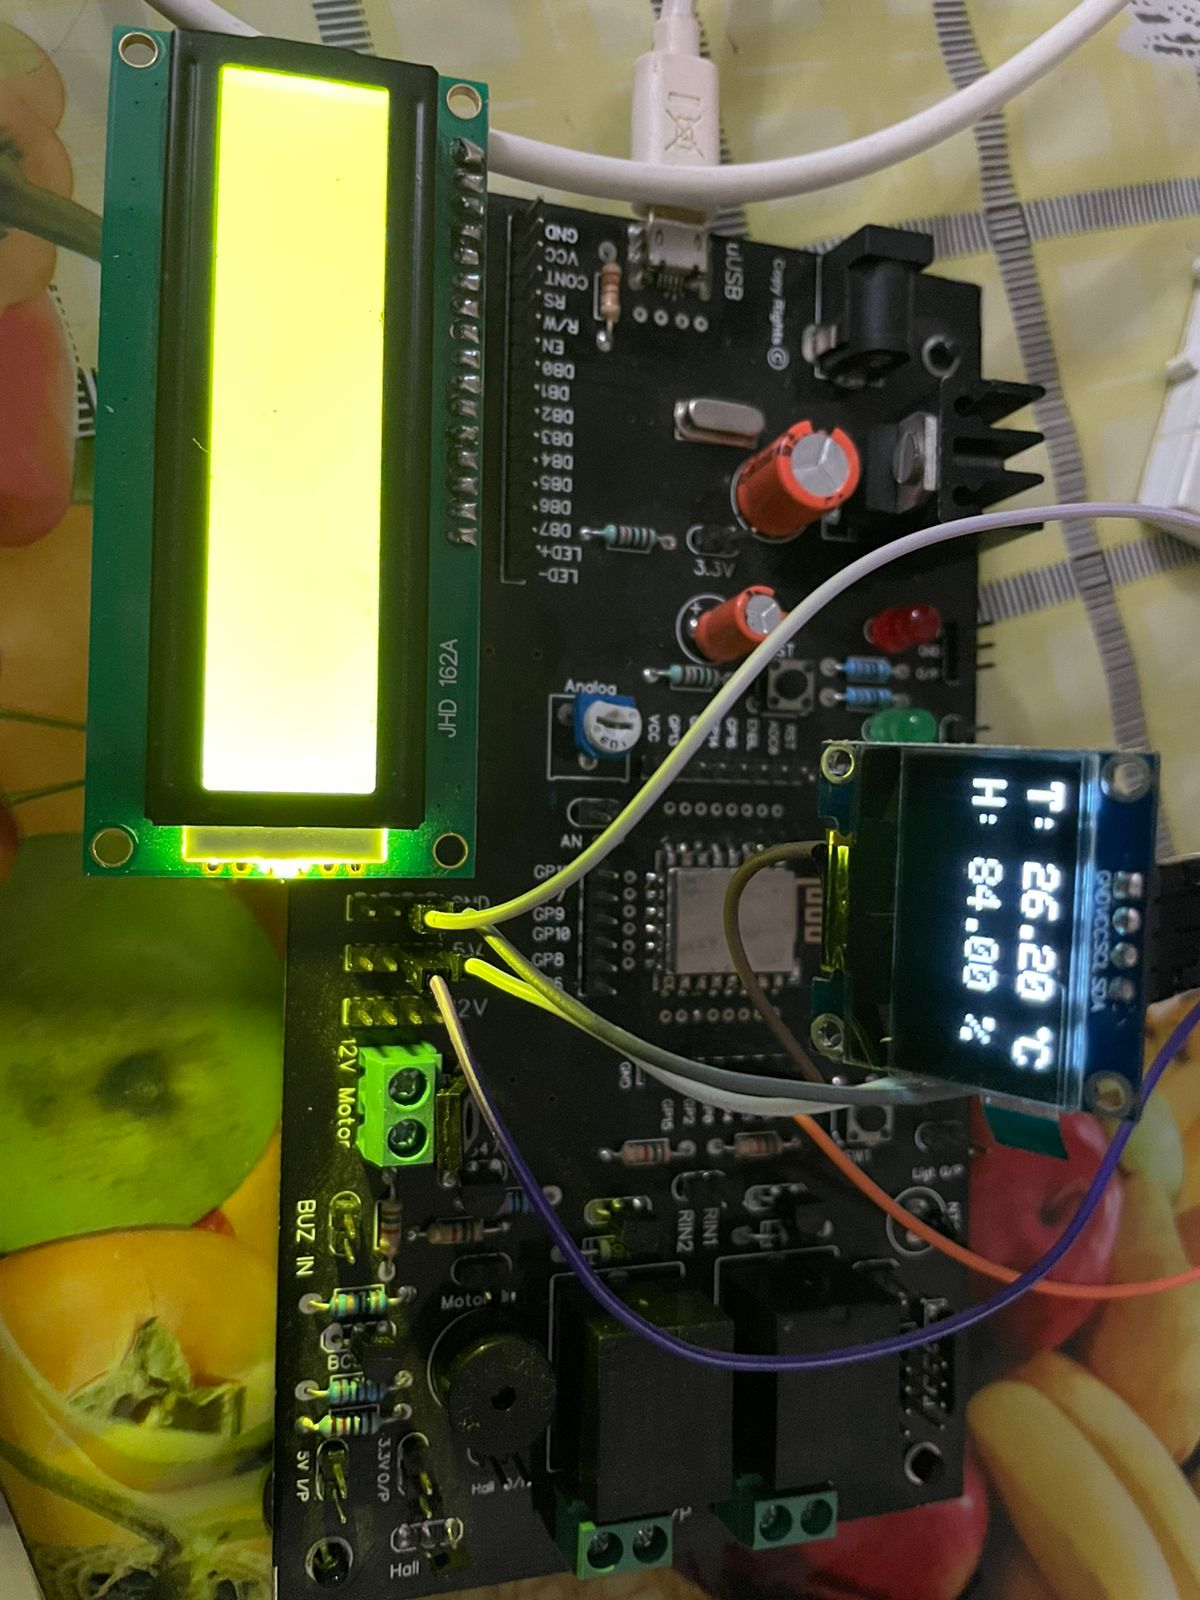
\includegraphics[width=15cm]{media/OLED.jpeg}
\centering
\caption{Display Values}
\end{figure}
\newpage
  \pagestyle{fancy}
  \thispagestyle{empty}
  \thispagestyle{plain}
  \fancyhf{}
  \lhead{ESP Async Web Server to Control Multiple Sensor Using NodeMCU $|$}
  \chead{}
  \rhead{Batch No.: 63}
  \rfoot{Page \thepage \hspace{1pt} of \pageref{LastPage}}
  \lfoot{Dept. of CSE, DSCE}
\renewcommand{\footrulewidth}{0.4pt}% 
\normalsize
\section*{Conclusion} 
This Internet of things is used widely in the nation. This makes it easier to control the temperature and humidity of any room or an organisation or in hospitals. This technology will help to monitor the patient's temperature as well as room temperature, humidity and patients ECG etc. 

These are but a few of the most widely used IoT applications worldwide. IoT may be used for an almost endless variety of purposes, particularly in combination with some other cutting-edge tools like automation. This is true especially considering since cheaper technology now allows devices to be used in multi - platforms and so build an interconnected Internet of Things (IoT) network.

Based on this carried out, many ideas have been brought up which are pointed out. Some of the papers have designed concepts which can be directly implemented and some others which can be altered according to the problem. In the existing system there is a need for manpower and synchronous usage of servers can be done. In this proposed system we have done the system as it works Asynchronously. This is the project of ESP Async webserver to control multiple sensor readings using NodeMCU.\\ 

\item \textbf{Future Enhancements:} we will fetch the data from the sensor and it will be stored in the cloud.In future we are planning to implement the alarm for the quick notification of high or low in the temperature.Simplifying the Web app login process by connecting the platform. It also provides good security.

\newpage
  \pagestyle{fancy}
  \thispagestyle{empty}
  \thispagestyle{plain}
  \fancyhf{}
  \lhead{ESPAsync Web Server to Control Multiple Sensor Reading Using NodeMCU $|$}
  \chead{}
  \rhead{Batch No.: 63}
  \rfoot{Page \thepage \hspace{1pt} of \pageref{LastPage}}
  \lfoot{Dept. of CSE, DSCE}
\renewcommand{\footrulewidth}{0.4pt}% 
\normalsize
\LARGE{\textbf{References}} 
\normalsize
\let\lbrack[
\let\rbrack]
\begin{enumerate}[\lbrack1{\rbrack}]
    \item Q. Yan, W. Huang, X. Luo, Q. Gong, and F. R. Yu, “A multi-level DDoS mitigation framework for the industrial Internet of Things,” IEEE Commun. Mag., vol. 56, no. 2, pp. 30–36, Feb. 2018.
    \item  D. Wu, J. Li, S. K. Das, J. Wu, Y. Ji, and Z. Li, “A novel distributed denial-of-service attack detection scheme for software defined networking environments,” in Proc. IEEE Int. Conf. Commun. (ICC), May 2018, pp. 1–6.
    \item C. Li, Z. Qin, E. Novak, and Q. Li, “Securing SDN infrastructure of IoT–fog networks from MitM attacks,” IEEE Internet Things J., vol. 4, no. 5, pp. 1156–1164,Oct. 2017.
    \item Y. Qiu and M. Ma, “Secure group mobility support for 6LoWPAN networks,” IEEE Internet Things J., vol. 5, no. 2, pp. 1131–1141, Apr. 2018.
    \item  D. B. Rawat and S. R. Reddy, “Software defined networking architecture, security and energy efficiency: A survey,” IEEE Commun. Surveys Tuts., vol. 19, no. 1, pp. 325–346, 1st Quart., 2017.
    \item E. Rescorla, H. Tschofenig, and N. Modadugu, “The datagram transport layer security (DTLS) protocol  version 1.3,” IETF, Fremont, CA, USA, draft-ietf-tls- dtls13-30, Nov. 2018. 
    \item  R. T. Tiburski, L. A. Amaral, E. de Matos, D. F. G. de Azevedo, and F. Hessel, “Evaluating the use of TLS and DTLS protocols in IoT middleware systems applied to E-health,” in Proc. 14th IEEE Annu. Consum.Commun. Netw. Conf. (CCNC), Jan. 2017, pp. 480–485.
    \item Third International Conference on Computing and Network Communications (CoCoNet’19)”A Novel MQTT Security framework In Generic IoT Model” Chintan Patel, Nishant Doshi Pandit Deendayal Petroleum University, Raisan-367002, Gujarat, India (2020).
    \item  U. Banerjee, C. Juvekar, S. H. Fuller, and A. P. Chandrakasan, “eeDTLS: Energy-efficient datagram transport layer security for the Internet of Things,” in Proc. IEEE Global Commun. Conf. (GLOBECOM),Dec. 2017, pp. 1–6. 
    \item N. Maheshwari and H. Dagale, “Secure communication and firewall architecture for IoT applications,” in Proc. 10th Int. Conf. Commun.Syst. Netw. (COMSNETS), Jan. 2018, pp. 328– 335.
    \item J. Cai et al., “A handshake protocol with unbalanced cost for wireless updating,” IEEE Access, vol. 6, pp. 18570–18581, 2018.
    \item A. Haroon, S. Akram, M. A. Shah, and A. Wahid, “E-Lithe: A lightweight secure DTLS for IoT,” in Proc. IEEE 86th Veh. Technol. Conf. (VTC-Fall), Sep. 2017, pp. 1–5.
    \item J. Park, H. Kwon, and N. Kang, “IoT—Cloud collaboration to establish a secure connection for lightweight devices,” Wireless Netw., vol. 23, no. 3, pp. 681–692, Apr. 2017.
    \item Marco Lombardi, Francesco Pascale, and Domenico Santaniello, “Internet of Things: A General Overview between Architectures, Protocols and Applications” (2021).
    \item Fatih Bakir, Rich Wolski, Chandra Krintz Univ. of California, Santa Barbara Gowri Sankar Ramachandran Univ. of Southern California, “Devices-as-Services: Rethinking Scalable Service Architectures for the Internet of Things” (2019). 
    \item W. Zhou, Y. Jia, A.   Peng, Y. Zhang, and P. Liu, “The effect of IoT new features on security and privacy: New threats, existing solutions, and challenges yet to be solved,” IEEE Internet Things J., vol. 6, no. 2, pp. 1606–1616, Apr. 2019.
\end{enumerate}
\newpage
  \pagestyle{fancy}
  \thispagestyle{empty}
  \thispagestyle{plain}
  \fancyhf{}
  \lhead{ESPAsync Web Server to Control Multiple Sensor Reading Using NodeMCU $|$}
  \chead{}
  \rhead{Batch No.: 63}
  \rfoot{Page \thepage \hspace{1pt} of \pageref{LastPage}}
  \lfoot{Dept. of CSE, DSCE}
\renewcommand{\footrulewidth}{0.4pt}% 
\normalsize
\section{Appendix} 
\subsection*{Sensor Code:} 
\subsection*{Sensor.ino} 
\definecolor{dkgreen}{rgb}{0,0.6,0}
\definecolor{gray}{rgb}{0.5,0.5,0.5}
\definecolor{mauve}{rgb}{0.58,0,0.82}

\lstset{frame=tb,
  language=Java,
  aboveskip=3mm,
  belowskip=3mm,
  showstringspaces=false,
  columns=flexible,
  basicstyle={\small\ttfamily},
  numbers=none,
  numberstyle=\tiny\color{gray},
  keywordstyle=\color{blue},
  commentstyle=\color{dkgreen},
  stringstyle=\color{mauve},
  breaklines=true,
  breakatwhitespace=true,
  tabsize=3
}
\begin{lstlisting}

void setup(){
  // Serial port for debugging purposes
  Serial.begin(115200);
  dht.begin();
    Serial.println();
  
  // Address 0x3C for 128x64, you might need to change this value (use an I2C scanner)
  if(!display.begin(SSD1306_SWITCHCAPVCC, 0x3C)) {
    Serial.println(F("SSD1306 allocation failed"));
    for(;;); // Don't proceed, loop forever
  }
  display.clearDisplay();
  display.setTextColor(WHITE);
  Serial.println("");
  Serial.println("Connected to WiFi"); 
  // Connect to Wi-Fi
  WiFi.begin(ssid, password);
  Serial.println("Connecting to WiFi");
  while (WiFi.status() != WL_CONNECTED) {
    delay(1000);
    Serial.println(".");
  }
server.begin();
  Serial.println("Web server running. Waiting for the ESP IP...");
  delay(10000);
  // Print ESP8266 Local IP Address
  Serial.println(WiFi.localIP());

  // Route for root / web page
  server.on("/", HTTP_GET, [](AsyncWebServerRequest *request){
    request->send_P(200, "text/html", index_html, processor);
  });
  server.on("/temperature", HTTP_GET, [](AsyncWebServerRequest *request){
    request->send_P(200, "text/plain", String(t).c_str());
  });
  server.on("/humidity", HTTP_GET, [](AsyncWebServerRequest *request){
    request->send_P(200, "text/plain", String(h).c_str());
  });

  // Start server
  server.begin();
}
 
void loop(){  
  unsigned long currentMillis = millis();
  if (currentMillis - previousMillis >= interval) {
    // save the last time you updated the DHT values
    previousMillis = currentMillis;
    // Read temperature as Celsius (the default)
    float newT = dht.readTemperature();
    // Read temperature as Fahrenheit (isFahrenheit = true)
    //float newT = dht.readTemperature(true);
    // if temperature read failed, don't change t value
    if (isnan(newT)) {
      Serial.println("Failed to read from DHT sensor!");
    }
    else {
      t = newT;
      Serial.println(t);
    }
    // Read Humidity
    float newH = dht.readHumidity();
    // if humidity read failed, don't change h value 
    if (isnan(newH)) {
      Serial.println("Failed to read from DHT sensor!");
    }
    else {
      h = newH;
      Serial.println(h);
    }
  }
}
\end{lstlisting}
\end{document}


